% Coffee Batch 3
\documentclass[10pt,twoside,footinclude=true,headinclude=true]{scrbook} % KOMA-Script book
\usepackage[LHE,T1]{fontenc}
\usepackage[paperheight=8.5in,paperwidth=5.5in,margin=0.3in,footskip=0.1in]{geometry}
\usepackage{hyperref}
\usepackage{graphicx}
\usepackage{watermark}
\usepackage[english]{babel}

\usepackage{fontspec}
\setmainfont{Roboto Mono}
\usepackage{xcolor}
\usepackage{colortbl}
\usepackage{wrapfig}
\usepackage{caption}
\usepackage{multicol}

\newfontfamily\smallcaps{Carrois Gothic SC}

\renewcommand*\raggedchapter{\centering}
\addtokomafont{pagenumber}{\scriptsize\normalfont}
\addtokomafont{chapter}{\Large\smallcaps}

\makeatletter
\def\@makeschapterhead#1{%
  %%%%%\vspace*{50\p@}%
  {\parindent \z@ \centering
    \smallcaps
    \interlinepenalty\@M
    \Large #1\par\nobreak
    \vskip 20\p@
  }}
\makeatother

\usepackage{titlesec}
\usepackage{ragged2e}
\usepackage{paracol}
\usepackage{transparent}
\usepackage{cancel}
\usepackage{tikz}
\usetikzlibrary{calc}

\title{Coffee Experiments}
\author{J. Jusman}

\newlength{\mysize}
\newcommand{\myfontsize}[1]{
  \setlength{\mysize}{#1pt}
  \fontsize{\mysize}{1.2\mysize}
  \selectfont
}

% TOC stuff.
\usepackage{tocloft}
\renewcommand{\cftchapleader}{\cftdotfill{\cftdotsep}}
\renewcommand{\cftchapfont}{\smallcaps}
\renewcommand{\cfttoctitlefont}{\smallcaps\Large}

% Better underlining.
\usepackage{ulem}
\usepackage{contour}
\renewcommand{\ULdepth}{1.3pt}
\contourlength{0.7pt}
\newcommand{\textul}[1]{%
  \uline{\phantom{#1}}%
  \llap{\contour{white}{#1}}%
}

% Helper functions.
\newcommand\blankpage{
    \clearpage
    \begingroup
      \null
      \thispagestyle{empty}%
      \addtocounter{page}{-1}%
      \hypersetup{pageanchor=false}%
      \clearpage
    \endgroup
}

\newcommand{\positionbox}[3]{
	\begin{tikzpicture}
		\node[inner sep=0pt] at ($(current page.north west) + (#1,-#2)$)
			{\transparent{0.1}\includegraphics[width=2in]{#3}};
	\end{tikzpicture}
}

\newcommand{\drawimage}[4]{
	\makebox[0pt][s]{
		\raisebox{#1}[0pt][0pt]{
			\transparent{#2}\includegraphics[width=#3]{#4}
		}
	}
}

\begin{document}

%-------------------------------------------------------------------------------
%	TITLE PAGE
%-------------------------------------------------------------------------------
\begin{titlepage}
\begin{center}

%\thiswatermark{\centering \put(0,-170) {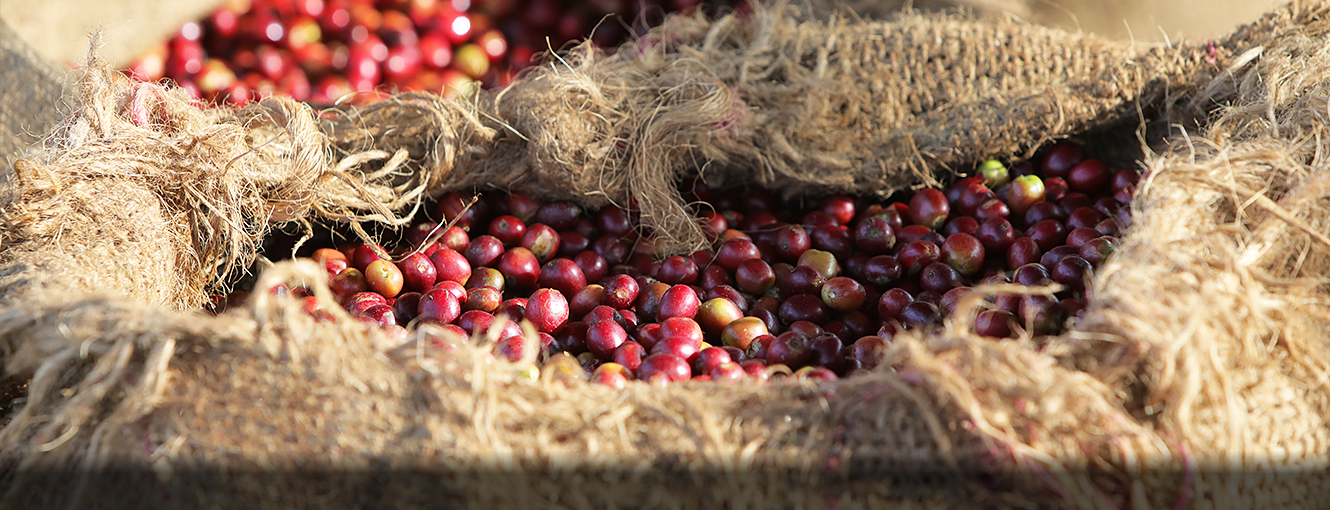
\includegraphics[width=10cm]{ethcoffeecherry}}}

\vspace*{3cm}
\large{\smallcaps{The Jusman Coffee Experiments}} \\
\bigskip
\Huge{\smallcaps{Fancy Batch \#3}} \\
\vspace{4.5cm}
\normalsize
Featured Vendor: \\
\medskip

\includegraphics[width=3cm]{sweet-marias-homepage-logo.png} \\
\vspace{5cm}

\textit{Merry Christmas and Happy New Year!} \\ \medskip % Subtitle

December 2019\ -- version 2.0 % Time and version

\vfill
\end{center}
\end{titlepage}
    
%\newpage
%\clearscrheadfoot
%\null

\pagenumbering{gobble}
\blankpage
\pagenumbering{arabic}

%-------------------------------------------------------------------------------
%	TOC
%-------------------------------------------------------------------------------
\tableofcontents 
\let\cleardoublepage=\clearpage % use \cleardoublepage here to avoid problems with pdfbookmark

%-------------------------------------------------------------------------------

\linespread{1.3}

%-------------------------------------------------------------------------------

\chapter*{Burundi Kayanza Masha Station}
\addcontentsline{toc}{chapter}{Burundi Kayanza Masha Station}
\markboth{}{}
 
\begin{addmargin}[2.2em]{2.2em}
\small
\justify
The level of sweetness ranks high (8.8!) - sugar in the raw, cream caramel, light brown sugar - with spiced flecks of cinnamon powder, hints of apple and pear and structuring acidity. City to Full City. Good for espresso.
\end{addmargin}

\centering
\vspace{2em}
\includegraphics[width=6cm]{charts/cupping.burundi-kayanza-masha-station-6075.png}
\includegraphics[width=6cm]{charts/flavor.burundi-kayanza-masha-station-6075.png}

\vspace{1em}
\begin{table}[htbp]
\myfontsize{7}
\hspace*{2.2em}
\begin{tabular}{ >{\raggedleft\arraybackslash}p{3.6cm}!{\color{lightgray}\vrule}p{7cm} }
\arrayrulecolor{lightgray}\hline
  Process Method & Wet Process \\
  \arrayrulecolor{lightgray}\hline
  Cultivar & Bourbon Types \\
  \arrayrulecolor{lightgray}\hline
  Farm Gate & Yes \\
  \arrayrulecolor{lightgray}\hline
  Region & Kayanza Province, Gatara Commune \\
  \arrayrulecolor{lightgray}\hline
  Processing & Wet Process (Washed) \\
  \arrayrulecolor{lightgray}\hline
  Drying Method & Raised Bed Sun-Dried \\
  \arrayrulecolor{lightgray}\hline
  Arrival date & January 2019 Arrival \\
  \arrayrulecolor{lightgray}\hline
  Lot size & 50 \\
  \arrayrulecolor{lightgray}\hline
  Bag size & 60 KG \\
  \arrayrulecolor{lightgray}\hline
  Packaging & GrainPro Liner \\
  \arrayrulecolor{lightgray}\hline
  Cultivar Detail & Bourbon \\
  \arrayrulecolor{lightgray}\hline
  Grade & A1 \\
  \arrayrulecolor{lightgray}\hline
  Appearance & .4 d/300gr, 16-18 Screen \\
  \arrayrulecolor{lightgray}\hline
  Roast Recommendations & City to Full City \\
  \arrayrulecolor{lightgray}\hline
  Type & Farm Gate \\
  \arrayrulecolor{lightgray}\hline
  Recommended for Espresso & Yes \\
  \arrayrulecolor{lightgray}\hline

\end{tabular}
\end{table}

%\centering
%\begin{tikzpicture}
%\draw (0,0) -- node [midway, fill=white] {\scriptsize Tom's Score} (2,0) -- (2,2) -- node[below, midway, yshift=-2em] {\Large 87.2} (0,2) -- (0,0);
%\draw (5,0) -- node [midway, fill=white] {\scriptsize My Score} (7,0) -- (7,2) -- (5,2) -- (5,0);
%\end{tikzpicture}

\newpage
\vspace*{-2.2em}
\raggedright
\normalsize
Farm Notes: \\
\myfontsize{8}
Masha Station is a coffee cherry collection site located in Kayanza, Burundi's northern province that borders neighboring Rwanda. The washing station acts as a central delivery site for a few thousand small holder famers who occupy the hills surrounding Masha. The name comes from the Kirundi word "amasho" that means "herds of cattle", which makes sense seeing that cattle herding just might rival coffee farming in the Masha region! Farmers grow mostly older bourbon types, the original coffee cultivar introduced to the area in the 1930s by Catholic monks traveling from the island of Reunion. Masha coffee washing station ("CWS") sits at just under 1700 meters above sea level, and many of the farmers have coffee planted much higher than this. They've been around since 1989, and in 2012 were top placement in Burundi Cup of Excellence competition, no small task. Masha roasts easily, very little roast color variance as you move from yellowing, to browning, and onto first crack. It helps that the sort is so good, with little to no trace of underripe coffee in the few hundred grams of coffee that we roasted. \\
\medskip
\normalsize
Cupping Notes: \\
\myfontsize{8}
This coffee from Masha has spiced sweetness in the dry fragrance, a mixture of baking spices and dark, raw sugars. City and City+ roasts smell very clean, and the wet aroma takes on characteristics of cinnamon-laced caramel. Masha is a clean tasting coffee too and an example of just how versatile Burundi coffees can be. They are a great alternative to clean and balanced Latin American coffees, offering rounded sweetness, mild top notes, and often structuring acidity like this lot from Masha does. The cup is sweet across a wide range of roasts, base flavors coming across like sugar in the raw, cream caramel, and light brown sugar. The level of sweetness ranks really high on our cupping spider graph (8.8!) and it's the one of the last characteristics I'm noting in the aftertaste. The coffee cools to spiced flecks of cinnamon powder up top, along with subtle hints of apple and pear at the lighter end of the roast spectrum, culminating in what reminds me of caramel apples. Full City roasting brings about roast tone as you'd expect, but is outweighed by sweetness, making for a silky semi-sweet chocolate flavor. Masha is well worth a run through your espresso machine if you're looking for a single origin espresso option that offers flavors of sweetened cocoa and spiced highlights. \\
\medskip
\normalsize
My Notes:

%-------------------------------------------------------------------------------

\chapter*{Burundi Kayanza Nemba Station}
\addcontentsline{toc}{chapter}{Burundi Kayanza Nemba Station}
 
\begin{addmargin}[2.2em]{2.2em}
\small
\justify
Tea and spice notes flourish in Nemba's brew, a chamomile floral aroma, spiced Darjeeling, along with a juicy lemon note. Acidity is brilliant like citrus and the tannic side of black tea. City to Full City.
\end{addmargin}

\centering
\vspace{2em}
\includegraphics[width=6cm]{charts/cupping.burundi-kayanza-nemba-station-5957.png}
\includegraphics[width=6cm]{charts/flavor.burundi-kayanza-nemba-station-5957.png}

\vspace{1em}
\begin{table}[htbp]
\myfontsize{7}
\hspace*{2.2em}
\begin{tabular}{ >{\raggedleft\arraybackslash}p{3.6cm}!{\color{lightgray}\vrule}p{7cm} }
\arrayrulecolor{lightgray}\hline
  Process Method & Wet Process \\
  \arrayrulecolor{lightgray}\hline
  Cultivar & Bourbon Types \\
  \arrayrulecolor{lightgray}\hline
  Farm Gate & Yes \\
  \arrayrulecolor{lightgray}\hline
  Region & Kayanza Province \\
  \arrayrulecolor{lightgray}\hline
  Processing & Wet Process (Washed) \\
  \arrayrulecolor{lightgray}\hline
  Drying Method & Raised Bed Sun Dried \\
  \arrayrulecolor{lightgray}\hline
  Arrival date & December 2018 Arrival \\
  \arrayrulecolor{lightgray}\hline
  Lot size & 60 \\
  \arrayrulecolor{lightgray}\hline
  Bag size & 60 KG \\
  \arrayrulecolor{lightgray}\hline
  Packaging & GrainPro liner \\
  \arrayrulecolor{lightgray}\hline
  Cultivar Detail & Bourbon \\
  \arrayrulecolor{lightgray}\hline
  Grade & A1 \\
  \arrayrulecolor{lightgray}\hline
  Appearance & .4 d/300gr, 16-18 Screen \\
  \arrayrulecolor{lightgray}\hline
  Roast Recommendations & City to Full City \\
  \arrayrulecolor{lightgray}\hline
  Type & Farm Gate \\
  \arrayrulecolor{lightgray}\hline

\end{tabular}
\end{table}

%\centering
%\begin{tikzpicture}
%\draw (0,0) -- node [midway, fill=white] {\scriptsize Tom's Score} (2,0) -- (2,2) -- node[below, midway, yshift=-2em] {\Large 87.9} (0,2) -- (0,0);
%\draw (5,0) -- node [midway, fill=white] {\scriptsize My Score} (7,0) -- (7,2) -- (5,2) -- (5,0);
%\end{tikzpicture}

\newpage
\vspace*{-2.2em}
\raggedright
\normalsize
Farm Notes: \\
\myfontsize{8}
Nemba Station is a coffee cherry collection and processing site located in Kayanza, Burundi's northern province that borders neighboring Rwanda. Farmers from surrounding "collines", or hill tops, deliver their harvest in whole cherry at the Nemba site, where it is then wet processed and then dried. Kayanza Province itself sits at 1800 meters above sea level, and the farms from the 15 hill tops that serve the Nemba Station top out at over 2000 meters. Farmers grow mostly older bourbon types, the original coffee cultivar introduced to the area in the 1930s by Catholic monks traveling from the island of Reunion. Nemba has been around since the early 1990s, and this year placed top 10 at the Burundi Cup of Excellence competition, no small task. Nemba roasts easily, very little roast color variance as you move from yellowing, to browning, and onto first crack. It helps that the sort is so good, with little to no trace of underripe coffee in the few hundred grams of coffee that we roasted.  \\
\medskip
\normalsize
Cupping Notes: \\
\myfontsize{8}
The dry fragrance of City roasts has a scent of sweet baking spices coupled with dried fruit, and a caramel corn candy hint. Full City is much more pungent and bittersweet as you might expect, but it still retains some of the caremely sweetness smelled in my lighter roast, showing promise as a darker roast option. A clove spice note comes up in the wet aroma, and breaking through the wetted crust releases a floral chamomile tea note. Light roasts have a lot of tea-like characteristics in the brewed coffee, not unlike most of the other Burundi's that we have right now. I picked up on chamomile floral aroma, and a spiced Darjeeling note is especially strong when the cup temperature cools off some. This, along with aspects of baking spices, is what causes these Burundi coffees to stand out amongst many other East African coffees (though finding parity with Rwandan coffee), and lends to a brisk cleanliness found in Nemba's finish. Fruited notes that are little more than accents when the coffee is hot, come way up after cooling off some, and mild cherry and red berry notes come through, as does a cherry cola flavor note. The acidic impressions are like citrus, and mouthfeel is on the tannic side in the finish. The sweetness holds up at Full City too, but bittering roast tones do much to counter this aspect. Not all is obfuscated by roast though, and the brewed coffee has flavors of high \% dark chocolate with roasted cacao nibs. \\
\medskip
\normalsize
My Notes:

%-------------------------------------------------------------------------------

\chapter*{Colombia Las Estrellas De Urrao}
\addcontentsline{toc}{chapter}{Colombia Las Estrellas De Urrao}
 
\begin{addmargin}[2.2em]{2.2em}
\small
\justify
Intense cup flavors, apple, dried plum, orange, and hibiscus tea. While I prefer the light and bright cups, dark berry notes flourish at Full City too. City to Full City.
\end{addmargin}

\centering
\vspace{2em}
\includegraphics[width=6cm]{charts/cupping.colombia-las-estrellas-de-urrao-6088.png}
\includegraphics[width=6cm]{charts/flavor.colombia-las-estrellas-de-urrao-6088.png}

\vspace{1em}
\begin{table}[htbp]
\myfontsize{7}
\hspace*{2.2em}
\begin{tabular}{ >{\raggedleft\arraybackslash}p{3.6cm}!{\color{lightgray}\vrule}p{7cm} }
\arrayrulecolor{lightgray}\hline
  Process Method & Wet Process \\
  \arrayrulecolor{lightgray}\hline
  Cultivar & Caturra Types, Modern Hybrids \\
  \arrayrulecolor{lightgray}\hline
  Farm Gate & Yes \\
  \arrayrulecolor{lightgray}\hline
  Region & Urrao, Antioquia \\
  \arrayrulecolor{lightgray}\hline
  Processing & Wet Process (Washed) \\
  \arrayrulecolor{lightgray}\hline
  Drying Method & Covered Sun-dried \\
  \arrayrulecolor{lightgray}\hline
  Arrival date & April 2019 Arrival \\
  \arrayrulecolor{lightgray}\hline
  Lot size & 13 \\
  \arrayrulecolor{lightgray}\hline
  Bag size & 70 KG \\
  \arrayrulecolor{lightgray}\hline
  Packaging & GrainPro Liner \\
  \arrayrulecolor{lightgray}\hline
  Cultivar Detail & Bourbon, Caturra, Typica \\
  \arrayrulecolor{lightgray}\hline
  Grade & Estate \\
  \arrayrulecolor{lightgray}\hline
  Appearance & .6 d/300gr, 15+ Screen \\
  \arrayrulecolor{lightgray}\hline
  Roast Recommendations & City to Full City \\
  \arrayrulecolor{lightgray}\hline
  Type & Farm Gate \\
  \arrayrulecolor{lightgray}\hline

\end{tabular}
\end{table}

%\centering
%\begin{tikzpicture}
%\draw (0,0) -- node [midway, fill=white] {\scriptsize Tom's Score} (2,0) -- (2,2) -- node[below, midway, yshift=-2em] {\Large 88.9} (0,2) -- (0,0);
%\draw (5,0) -- node [midway, fill=white] {\scriptsize My Score} (7,0) -- (7,2) -- (5,2) -- (5,0);
%\end{tikzpicture}

\newpage
\vspace*{-2.2em}
\raggedright
\normalsize
Farm Notes: \\
\myfontsize{8}
This Urrao microlot is made up of 10 of the highest scoring coffee from producers in Urrao, Antioquia. The Penderisco river runs through the main valley leading to Urrao, and the growing areas where these coffees are from - San Carlos, Pavón, La Cartagena and Arenales. Most of these farms are marked by steep, red clay slopes that drop precipitously to the creek lined floors below. These farmers are part of an allied producer group in the area who allow us and our local partner to use their cupping lab in order to and evaluate and separate out the highest scoring lots. We pay a premium for this level of access, the lion's share of that payment going back directly to the coffee producer. This is a blend of a Caturra and an heirloom referred to locally as "Chiroso", thought to be a natural mutation of Caturra. "Chiroso" has elongated, narrow-shaped cherries/seeds that look an awful lot like Typica, and are fairly easy to pick out of the green based on this canoe-like shape (have a look through your green and you'll see what I mean). Coffee is processed at home and subjected to long fermentation times, due in part to the cold, natural spring water that is used for processing. That helps explain a more fruit-forward cup quality that we tend to see in coffees from Urrao. The valley floor is roughly 1800 meters above sea level, and coffee is planted all the way up to 2100 meters. \\
\medskip
\normalsize
Cupping Notes: \\
\myfontsize{8}
You really get a sense of the intense sweetness when grinding this Urrao coffee. The fragrance has dark dried fruit smells (fig, or prune?) with baked muffin-like honeyed sweetness that is near floral. Aromatically, Las Estrellas de Urrao shows intense dark fruited sweetness that has the rustic side of dried fruits and spiced notes integrated in the background. The fruited flavors displayed in the cup help define the coffee's sweetness, and also carry a dried fruit/rustic appeal. The intensity increases as the coffee cools down some, flavor notes of red apple, plum, pulpy orange juice were noted, along with a refreshing, somewhat floral hibiscus tea note in the finish. This one's a showstopper for sure, and while I prefer the light and bright approach, where a citric impression is undeniable, my Full City roast drew out delicious dark blueberry flavors that fit right in with the bittersweet chocolate roast tone flowing from front to back of the cup profile. \\
\medskip
\normalsize
My Notes:

%-------------------------------------------------------------------------------

\chapter*{Ethiopia Organic Dry Process Sidama Shantawene}
\addcontentsline{toc}{chapter}{Ethiopia Organic Dry Process Sidama Shantawene}
 
\begin{addmargin}[2.2em]{2.2em}
\small
\justify
A heavy-handed dry process cup, notes of blueberry, grape, cranberry juice, honeydew, stone fruit accents and tart citrus hints. A wine-like, sweet coffee on the cleaner side for natural. City to Full City. Wild espresso.
\end{addmargin}

\centering
\vspace{3mm}
\includegraphics[width=6cm]{charts/cupping.ethiopia-organic-dry-process-sidama-shantawene-6289.png}
\includegraphics[width=6cm]{charts/flavor.ethiopia-organic-dry-process-sidama-shantawene-6289.png}

\vspace{1mm}
\begin{table}[htbp]
\myfontsize{7}
\hspace*{2.2em}
\begin{tabular}{ >{\raggedleft\arraybackslash}p{3.6cm}!{\color{lightgray}\vrule}p{7cm} }
\arrayrulecolor{lightgray}\hline
  Process Method & Dry Process \\
  \arrayrulecolor{lightgray}\hline
  Cultivar & Heirloom Types \\
  \arrayrulecolor{lightgray}\hline
  Farm Gate & Yes \\
  \arrayrulecolor{lightgray}\hline
  Region & Shantawene, Sidama \\
  \arrayrulecolor{lightgray}\hline
  Processing & Dry Process (Natural) \\
  \arrayrulecolor{lightgray}\hline
  Drying Method & Raised Bed Sun-Dried \\
  \arrayrulecolor{lightgray}\hline
  Arrival date & September 2019 Arrival \\
  \arrayrulecolor{lightgray}\hline
  Lot size & 100 \\
  \arrayrulecolor{lightgray}\hline
  Bag size & 60 KG \\
  \arrayrulecolor{lightgray}\hline
  Packaging & GrainPro Liner \\
  \arrayrulecolor{lightgray}\hline
  Cultivar Detail & Heirloom Cultivars \\
  \arrayrulecolor{lightgray}\hline
  Grade & Grade 1 \\
  \arrayrulecolor{lightgray}\hline
  Appearance & .8 d per 300 gr; 14+ screen - mainly partial quakers, there are a lot of small beans too (not a defect) \\
  \arrayrulecolor{lightgray}\hline
  Roast Recommendations & City to Full City - take care roasting dark as the small beans can roast faster than the others when taken too fast \\
  \arrayrulecolor{lightgray}\hline
  Type & Farm Gate, Certified Coffees \\
  \arrayrulecolor{lightgray}\hline
  Recommended for Espresso & Yes \\
  \arrayrulecolor{lightgray}\hline
  Certifications & Organic \\
  \arrayrulecolor{lightgray}\hline

\end{tabular}
\end{table}

%\centering
%\begin{tikzpicture}
%\draw (0,0) -- node [midway, fill=white] {\scriptsize Tom's Score} (2,0) -- (2,2) -- node[below, midway, yshift=-2em] {\Large 93} (0,2) -- (0,0);
%\draw (5,0) -- node [midway, fill=white] {\scriptsize My Score} (7,0) -- (7,2) -- (5,2) -- (5,0);
%\end{tikzpicture}

\newpage
\vspace*{-2.2em}
\linespread{1.2}
\raggedright
\normalsize
Farm Notes: \\
\myfontsize{7.8}
This coffee is one of two lots being sold under the "Shantawene" name, the other being a fantastic wet process coffee also available now. Both coffees come from a privately owned farm and processing site near Shantawene Village, tucked away in the Bombe mountains of Ethiopia's Sidama growing region. Along with coffee from their own farm called "Daye Bensa", they are buying and processing coffee from local farmers from three different growing areas nearby - Shantawene, Bombe and Keramo villages. The samples we tasted from all three scored high and we wound up buying wet and dry process lots from all of them (the others should be available early 2020). This lot is a mix of coffees harvested from their own farm and outgrowers around Shantawene village. It's certified organic too, which means that they go to great lengths to register every small farmer who they buy from and certify that organic agricultural practices are being employed at the farm level (they're also Rain Forest Alliance and UTZ certified, but we only brought in with the organic certificate). The farm and outgrowers are growing Ethiopian heirlooms and altitude ranges from just under 2000 meters to 2100 meters above sea level. It's worth noting that the screen size is on the small side too. The majority of the coffee is 15+, but we are spotting quite a few 14 screen beans in there too. The biggest concern here is that these smaller, lower density beans will roast faster than the largest coffee. While that can be true, we found that either sticking to City to City+ roast range or slowing down the last leg of the roast helps keep the small beans from charring and darker 'roast' flavors at bay. \\
\medskip
\normalsize
Cupping Notes: \\
\myfontsize{7.8}
Dry process Ethiopias are perhaps some of the most complex coffees we carry, and this lot from Shantawene is a testament to that. It's on the cleaner side of the spectrum too, fruit and berry flavors are fairly refined, and even display a floral aroma that adds a delicate quality to the cup profile, though I'd hardly call this natural "delicate"! At City and City+ the cup is heavy handed, with flavors notes of berry and grape, sweetened cranberry juice, honeydew melon and stone fruit accents. Aspects of tart fruit flavors cut through the complex cup profile and add an acidic impression and structuring effect to the array of wild fruit flavors. Shantawene displays some wine-like, ferment flavors too, but nothing in the 'booze'/alcohol realm that might indicate the coffee sat on the drying beds too long, and they're much more like the plum flavors of a young wine. Full City roasts bring out the berry tones and a lingering blueberry flavor is easily ID'd and comes with something akin to tart fruit skins. Full City roasting is a little tricky due to the small screen size of some of the beans (they look like 14 screen). If you have the means to control heat, try pulling back a little before or at the fist audible snaps. Slowing down the roast will help to keep from charring the tiniest beans. If you're roasting in a popper, I'd try shooting for City/City+ max and call it a day. Lighter roasts were my personal favorite anyway. And as espresso? I'm giving it my recommendation with the disclaimer that it's a wild ride, jam packed with the aforementioned fruit flavors distilled to a tart point that is puckering and slightly sharp when roasted any lighter than Full City. Not for everyone, but I sure love it. \\
\medskip
\normalsize
My Notes:
\linespread{1.3}

%-------------------------------------------------------------------------------

\chapter*{Ethiopia Organic Sidama Shantawene Village}
\addcontentsline{toc}{chapter}{Ethiopia Organic Sidama Shantawene Village}
 
\begin{addmargin}[2.2em]{2.2em}
\small
\justify
SO sweet (9.6!), floral honey and honey comb, citrus high tones, honey tangerine and Valencia orange, light touches of jasmine, fresia, berry and baking spice. City to City+
\end{addmargin}

\centering
\vspace{2em}
\includegraphics[width=6cm]{charts/cupping.ethiopia-organic-sidama-shantawene-village-6285.png}
\includegraphics[width=6cm]{charts/flavor.ethiopia-organic-sidama-shantawene-village-6285.png}

\vspace{1em}
\begin{table}[htbp]
\myfontsize{7}
\hspace*{2.2em}
\begin{tabular}{ >{\raggedleft\arraybackslash}p{3.6cm}!{\color{lightgray}\vrule}p{7cm} }
\arrayrulecolor{lightgray}\hline
  Process Method & Wet Process \\
  \arrayrulecolor{lightgray}\hline
  Cultivar & Heirloom Types \\
  \arrayrulecolor{lightgray}\hline
  Farm Gate & Yes \\
  \arrayrulecolor{lightgray}\hline
  Region & Shantawene Village, Sidama \\
  \arrayrulecolor{lightgray}\hline
  Processing & Wet Process \\
  \arrayrulecolor{lightgray}\hline
  Drying Method & Raised Bed Sun-Dried \\
  \arrayrulecolor{lightgray}\hline
  Arrival date & September 2019 Arrival \\
  \arrayrulecolor{lightgray}\hline
  Lot size & 120 \\
  \arrayrulecolor{lightgray}\hline
  Bag size & 60 KG \\
  \arrayrulecolor{lightgray}\hline
  Packaging & GrainPro Liner \\
  \arrayrulecolor{lightgray}\hline
  Cultivar Detail & Heirloom Cultivars \\
  \arrayrulecolor{lightgray}\hline
  Grade & Grade 1 \\
  \arrayrulecolor{lightgray}\hline
  Appearance & .5 d/300gr, 14+ Screen - a mix of screen sizes as small as 14 \\
  \arrayrulecolor{lightgray}\hline
  Roast Recommendations & City to City+ \\
  \arrayrulecolor{lightgray}\hline
  Type & Farm Gate \\
  \arrayrulecolor{lightgray}\hline
  Certifications & Organic \\
  \arrayrulecolor{lightgray}\hline

\end{tabular}
\end{table}

%\centering
%\begin{tikzpicture}
%\draw (0,0) -- node [midway, fill=white] {\scriptsize Tom's Score} (2,0) -- (2,2) -- node[below, midway, yshift=-2em] {\Large 92} (0,2) -- (0,0);
%\draw (5,0) -- node [midway, fill=white] {\scriptsize My Score} (7,0) -- (7,2) -- (5,2) -- (5,0);
%\end{tikzpicture}

\newpage
\vspace*{-2.2em}
\raggedright
\normalsize
Farm Notes: \\
\myfontsize{8}
This coffee is one of two lots being sold under the "Shantawene" name, the other being a fantastic dry process coffee also available now. Both coffees come from a privately owned farm and processing site in Shantawene Village, tucked away in the Bombe mountains of Ethiopia's Sidama growing region. Along with coffee from their own estate called "Daye Bensa", they are buying and processing coffee from local farmers from three different growing areas nearby - Shantawene, Bombe and Keramo villages. The samples we tasted from all three rated high and we wound up buying wet and dry process lots from all of them (the others should be available early 2020). This lot is a mix of coffees harvested from their own farm and outgrowers around Shantawene village. It's certified organic too, which means that they go to great lengths to register every small farmer who they buy from and certify that organic agricultural practices are being employed at the farm level (they're also Rain Forest Alliance and UTZ certified, but we only brought in with the organic certificate). The farm and outgrowers are growing Ethiopian heirlooms and altitude ranges from just under 2000 meters to 2100 meters above sea level. It's worth noting that the screen size is on the small side too. The majority of the coffee is 15+, but we are spotting quite a few 14 screen beans in there too.The biggest concern here is that these smaller, lower density beans will roast faster than the largest coffee. While that can be true, we found that either sticking to City to City+ roast range or slowing down the last leg of the roast, helps keep the small beans from charring and darker 'roast' flavors at bay. \\
\medskip
\normalsize
Cupping Notes: \\
\myfontsize{8}
This wet process lot from Shantawene has the sweetness of ginger snap cookies in the dry grounds, light touches of sweet spice, honey and dried fruit. The wet aroma has honey appeal, not so much floral in a 'jasmine' way like you might expect from Guji, but more of a raw honey like floral. It's incredibly sweet smelling and has the intensity of honey in the comb. This translates in the cup too and City and City+ roasts have a sweet honey base flavor that resonates in the finish (sweetness scored a whopping 9.6!). A vibrant citrus note shines bright in lighter roasts, and with that intesne underlying sweetness underneath, sweet citrus like honey tangerine and Valencia oranges (the juicing kind) come to mind. As the coffee cools off you do catch a glimpse of fresh flowers, perfumed accents of start jasmine and fresia, both potent flowers for sure, but not incredibly potent in comparison to the other cup highlights. Give it some time after brewing and darker fruit and berry flavors start to surface, as do soft baking spice finishing highlights. An incredibly clean Ethiopian coffee with competition level sweetness when roasted light to medium. We also happen to have a dry process lot of this coffee available which presents a unique opportunity to the same coffee from the same site processed two different ways.  \\
\medskip
\normalsize
My Notes:

%-------------------------------------------------------------------------------

\chapter*{Flores Laga Lizu Gnung Waja Mala}
\addcontentsline{toc}{chapter}{Flores Laga Lizu Gnung Waja Mala}
 
\begin{addmargin}[2.2em]{2.2em}
\small
\justify
Waja Mala has a bran muffin aspect in aroma, with flavors of turbinado sugar, walnut, raisin and the bittersweetness of flourless chocolate torte. City to Full City.
\end{addmargin}

\centering
\vspace{2em}
\includegraphics[width=6cm]{charts/cupping.flores-laga-lizu-gnung-waja-mala-6054.png}
\includegraphics[width=6cm]{charts/flavor.flores-laga-lizu-gnung-waja-mala-6054.png}

\vspace{1em}
\begin{table}[htbp]
\myfontsize{7}
\hspace*{2.2em}
\begin{tabular}{ >{\raggedleft\arraybackslash}p{3.6cm}!{\color{lightgray}\vrule}p{7cm} }
\arrayrulecolor{lightgray}\hline
  Process Method & Wet Process \\
  \arrayrulecolor{lightgray}\hline
  Cultivar & Typica Types, Modern Hybrids \\
  \arrayrulecolor{lightgray}\hline
  Farm Gate & Yes \\
  \arrayrulecolor{lightgray}\hline
  Region & Waja Mala \\
  \arrayrulecolor{lightgray}\hline
  Processing & Wet Process (Washed) \\
  \arrayrulecolor{lightgray}\hline
  Drying Method & Patio Sun-Dried \\
  \arrayrulecolor{lightgray}\hline
  Arrival date & December 2018 Arrival \\
  \arrayrulecolor{lightgray}\hline
  Lot size & 28 \\
  \arrayrulecolor{lightgray}\hline
  Bag size & 60 KG \\
  \arrayrulecolor{lightgray}\hline
  Packaging & GrainPro Liner \\
  \arrayrulecolor{lightgray}\hline
  Cultivar Detail & S795, Typica \\
  \arrayrulecolor{lightgray}\hline
  Grade & Grade 1 \\
  \arrayrulecolor{lightgray}\hline
  Appearance & .7 d/300gr, 16-18 Screen \\
  \arrayrulecolor{lightgray}\hline
  Roast Recommendations & City to Full City \\
  \arrayrulecolor{lightgray}\hline
  Type & Farm Gate \\
  \arrayrulecolor{lightgray}\hline

\end{tabular}
\end{table}

%\centering
%\begin{tikzpicture}
%\draw (0,0) -- node [midway, fill=white] {\scriptsize Tom's Score} (2,0) -- (2,2) -- node[below, midway, yshift=-2em] {\Large 86} (0,2) -- (0,0);
%\draw (5,0) -- node [midway, fill=white] {\scriptsize My Score} (7,0) -- (7,2) -- (5,2) -- (5,0);
%\end{tikzpicture}

\newpage
\vspace*{-2.2em}
\raggedright
\normalsize
Farm Notes: \\
\myfontsize{8}
This coffee called "Waja Mala" is from a small cooperative near the village of Rada Bata. "Gunung" translates roughly to "peak" or "hill", which in the case of Waja Mala, is one of the higher elevations in this volcanic region. They're part of a coordinated effort to unite coffee growers from neighboring villages in a coffee farmers cooperative, whom we've been introduced to through an intermediary working in the region. Much of the kinship groups in these areas are matrilineal, with land being passed through women. Because of this, you see a lot more women in leadership positions at the farm and cooperative levels. This is an all female-run coop and we were introduced to their coffee through a Q-grader we're working with in the region, who also happens to have a leadership role at this coop in Waja Mala. Most of the coffees are processed on hand cranked or motorized depulping machines on the farm, fermentation in buckets or small tanks, and then drying on raised drying beds. Because of the nutrient rich soils, they are able to grow coffee using fully organic farm practices, though they are not certified at this time. \\
\medskip
\normalsize
Cupping Notes: \\
\myfontsize{8}
The dry fragrance has a bran muffin smell at City+ roast level, like honey-sweet baked goods, and with a ginger powder accent. Pouring the hot water brings on a much more bittersweet side of Waja Mala, still with the dark sweetness too, but along with bittering cocoa powder and malted cocoa on the break. Waja Mala brews well at a wide range of roasts too. City and City+ bring out raw sugar sweetness that has a flavor of turbinado sugar, and flanked by a walnut note that adds both a sweet nut tone and slight bittering walnut skin mouthfeel. Deeper roasting brings bittersweetness to its climax though developing all the way to 2nd cracks will usher in ashy/bittering tones that tend to obfuscate sweetness. Full City is a nice stopping point, and has that bitter-to-sweet flavor that you find in flourless chocolate torte, and a subtle raisin note comes into view in the finish. \\
\medskip
\normalsize
My Notes:

%-------------------------------------------------------------------------------

\chapter*{Guatemala Proyecto Xinabajul Tujlate}
\addcontentsline{toc}{chapter}{Guatemala Proyecto Xinabajul Tujlate}
 
\begin{addmargin}[2.2em]{2.2em}
\small
\justify
Fruited aroma, notes of raw sugar, apple and orange are connected by bracing, tart acidity. Sweetness sticks around in the finish, peppered by an accent of malted milk powder. City to Full City+.
\end{addmargin}

\centering
\vspace{2em}
\includegraphics[width=6cm]{charts/cupping.guatemala-proyecto-xinabajul-tujlate-6162.png}
\includegraphics[width=6cm]{charts/flavor.guatemala-proyecto-xinabajul-tujlate-6162.png}

\vspace{1em}
\begin{table}[htbp]
\myfontsize{7}
\hspace*{2.2em}
\begin{tabular}{ >{\raggedleft\arraybackslash}p{3.6cm}!{\color{lightgray}\vrule}p{7cm} }
\arrayrulecolor{lightgray}\hline
  Process Method & Wet Process \\
  \arrayrulecolor{lightgray}\hline
  Cultivar & Caturra Types, Bourbon Types, Typica Types \\
  \arrayrulecolor{lightgray}\hline
  Farm Gate & Yes \\
  \arrayrulecolor{lightgray}\hline
  Region & Santiago Chimaltenango, Huehuetenango \\
  \arrayrulecolor{lightgray}\hline
  Processing & Wet Process (Washed) \\
  \arrayrulecolor{lightgray}\hline
  Drying Method & Patio Sun-Dried \\
  \arrayrulecolor{lightgray}\hline
  Arrival date & June 2019 Arrival \\
  \arrayrulecolor{lightgray}\hline
  Lot size & 10 \\
  \arrayrulecolor{lightgray}\hline
  Bag size & 69 KG \\
  \arrayrulecolor{lightgray}\hline
  Packaging & GrainPro Liner \\
  \arrayrulecolor{lightgray}\hline
  Cultivar Detail & Bourbon, Caturra, Catuai, Typica \\
  \arrayrulecolor{lightgray}\hline
  Grade & SHB EP \\
  \arrayrulecolor{lightgray}\hline
  Appearance & .5 d/300gr, 16-18 Screen \\
  \arrayrulecolor{lightgray}\hline
  Roast Recommendations & City to Full City+ \\
  \arrayrulecolor{lightgray}\hline
  Type & Farm Gate \\
  \arrayrulecolor{lightgray}\hline

\end{tabular}
\end{table}

%\centering
%\begin{tikzpicture}
%\draw (0,0) -- node [midway, fill=white] {\scriptsize Tom's Score} (2,0) -- (2,2) -- node[below, midway, yshift=-2em] {\Large 87.5} (0,2) -- (0,0);
%\draw (5,0) -- node [midway, fill=white] {\scriptsize My Score} (7,0) -- (7,2) -- (5,2) -- (5,0);
%\end{tikzpicture}

\newpage
\vspace*{-2.2em}
\raggedright
\normalsize
Farm Notes: \\
\myfontsize{8}
"Tujlate" is the village where this coffee is from, located in the Municipality of Santiago Chimaltenango. Not to be confused with "Chimaltenango" near Antigua, this area is in Huehuetenango highland region not far from San Pedro Necta (remember Finca Rosma?). It's actually a single producer lot from farmer Juan Ramirez, whose coffee we came across on a visit to Huehue last Spring. It was 1 of at least 100 samples during a day of cupping in Huehue town, and the underlying fruited qualities stood out from the pack. We haven't visited his farm or this particular town but hope to see more coffee from Santiago Chimaltenango in the 2020 harvest season. Altitude in the town is 1,786 meters and it only goes up from there. Like so many farmers in this area, Juan Ramirez is likely growing a mix of Caturra and Catuai with some Typica mixed in. \\
\medskip
\normalsize
Cupping Notes: \\
\myfontsize{8}
First and foremost, I pick up on sweet sugar browning smells in the dry fragrance, like raw sugar toasting in a pan. But there're strong indications of fruit too, at least for a washed Guatemalan coffee. It's an aspect that seems to build with each step in our cup assessment: from dry grounds, to wet aroma, and the final fruited flavors in the brewed coffee. At City roast level, a juicy green apple flavor is noted in the background amidst resonant raw sugar sweetness and mild bittering roast tone. The cup is balanced in terms of sweet and bitter roast flavors , and at this roast level, apple and orange top notes are tethered to the underlying bittersweet profile by bracing, tart acidity. The finish is sweet and there's a malted milk powder note in the long aftertaste. Full City roasting leads to a much more cocoa-centered brew, a flavor of dark chocolate with a bittering bite up front, leads into sweet chocolate notes like Tootsie Roll, along with cooked fruit hints in the middle and finish. \\
\medskip
\normalsize
My Notes:

%-------------------------------------------------------------------------------

\chapter*{Guatemala Xinabajul Antonio Castillo}
\addcontentsline{toc}{chapter}{Guatemala Xinabajul Antonio Castillo}
 
\begin{addmargin}[2.2em]{2.2em}
\small
\justify
Layered sweetness - caramelizing sugars, butterscotch, and molasses - hints of apple and pear, a tart malic acidity. Full City produces opaque cocoa roast tones balanced by a sturdy sweet base. City to Full City+. Good for espresso.
\end{addmargin}

\centering
\vspace{2em}
\includegraphics[width=6cm]{charts/cupping.guatemala-xinabajul-antonio-castillo-6150.png}
\includegraphics[width=6cm]{charts/flavor.guatemala-xinabajul-antonio-castillo-6150.png}

\vspace{1em}
\begin{table}[htbp]
\myfontsize{7}
\hspace*{2.2em}
\begin{tabular}{ >{\raggedleft\arraybackslash}p{3.6cm}!{\color{lightgray}\vrule}p{7cm} }
\arrayrulecolor{lightgray}\hline
  Process Method & Wet Process \\
  \arrayrulecolor{lightgray}\hline
  Cultivar & Caturra Types, Bourbon Types, Typica Types \\
  \arrayrulecolor{lightgray}\hline
  Farm Gate & Yes \\
  \arrayrulecolor{lightgray}\hline
  Region & Bojonalito Ixtaltilar, La Libertad, Huehuetenango \\
  \arrayrulecolor{lightgray}\hline
  Processing & Wet Process (Washed) \\
  \arrayrulecolor{lightgray}\hline
  Drying Method & Patio Sun-Dried \\
  \arrayrulecolor{lightgray}\hline
  Arrival date & June 2019 Arrival \\
  \arrayrulecolor{lightgray}\hline
  Lot size & 20 \\
  \arrayrulecolor{lightgray}\hline
  Bag size & 69 KG \\
  \arrayrulecolor{lightgray}\hline
  Packaging & GrainPro Liner \\
  \arrayrulecolor{lightgray}\hline
  Cultivar Detail & Bourbon, Caturra, Catuai, Typica \\
  \arrayrulecolor{lightgray}\hline
  Grade & SHB EP \\
  \arrayrulecolor{lightgray}\hline
  Appearance & .4 d/300gr, 16-18 Screen \\
  \arrayrulecolor{lightgray}\hline
  Roast Recommendations & City to Full City+ \\
  \arrayrulecolor{lightgray}\hline
  Type & Farm Gate \\
  \arrayrulecolor{lightgray}\hline
  Recommended for Espresso & Yes \\
  \arrayrulecolor{lightgray}\hline

\end{tabular}
\end{table}

%\centering
%\begin{tikzpicture}
%\draw (0,0) -- node [midway, fill=white] {\scriptsize Tom's Score} (2,0) -- (2,2) -- node[below, midway, yshift=-2em] {\Large 87.8} (0,2) -- (0,0);
%\draw (5,0) -- node [midway, fill=white] {\scriptsize My Score} (7,0) -- (7,2) -- (5,2) -- (5,0);
%\end{tikzpicture}

\newpage
\vspace*{-2.2em}
\raggedright
\normalsize
Farm Notes: \\
\myfontsize{8}
Looking back at the last 4 years of Guatemala cupping notes and Antonio's name is all over them. 5 bags here, and as many as 10 bags one year, but always folded in to a regional blend. I don't see a single coffee lot from him that we didn't approve. Well, this year we're happy to bring in 20 full bags of Antonio's coffee, a record! It's a good chunk of coffee from any single producer and certainly needed to be kept separate so that we can offer on it's own. Antonio's farm is located in the community of Bojonalito, a small village within the larger municipality of La Libertad, Huehuetenango. His farm is situated right around 1700 meters above sea level and planted in a mix of Bourbon, Caturra and Typica. The coffee is wet process, meaning depulped and then using fermeentation to remove the sticky layer of fruit before moving to the drying patio. The dry parchment is then transported to Huehue town where it is dry milled and prepared for the final transport to the US. Antonio is part of our "Proyecto Xinabajul" in Huehuetenango, which you can read an in-depth and detailed description of the HERE. \\
\medskip
\normalsize
Cupping Notes: \\
\myfontsize{8}
This lot from Antonio Castillo cupped so sweet at both City and Full City roast levels. In fact, my darker of the two roasts was very close to 2nd snaps (36F degrees development post 1stC). And while loaded with heavy bittering cocoa roast flavors, the underlying sweetness keeps the cup well in balance. Fragrance and aroma have butterscotch-like sweet smells, layered with toffee nut and smokey wisps of browned sugars. The cup at City has a pear note as it cools and moderate tart acidic impressions. Butterscotch is also a dominant flavor in light to middle roasts, along with raw sugar and a molasses hint. Full City roasts produce opaque cocoa roast tones balanced by a sturdy sweet base of burned sugar flavors. Definitely a prime candidate for a chocolate-centered espresso shot too. \\
\medskip
\normalsize
My Notes:

%-------------------------------------------------------------------------------

\chapter*{Kenya Kiambu Dagitu}
\addcontentsline{toc}{chapter}{Kenya Kiambu Dagitu}
 
\begin{addmargin}[2.2em]{2.2em}
\small
\justify
Dagitu is a fruited coffee with flavor notes falling into the fleshy fruit (plum, grape, cranberry, etc) and citrus categories, with red fruit punch thrown in there too. Sweet, clean and lively acidity. City to Full City.
\end{addmargin}

\centering
\vspace{2em}
\includegraphics[width=6cm]{charts/cupping.kenya-kiambu-dagitu-6259.png}
\includegraphics[width=6cm]{charts/flavor.kenya-kiambu-dagitu-6259.png}

\vspace{1em}
\begin{table}[htbp]
\myfontsize{7}
\hspace*{2.2em}
\begin{tabular}{ >{\raggedleft\arraybackslash}p{3.6cm}!{\color{lightgray}\vrule}p{7cm} }
\arrayrulecolor{lightgray}\hline
  Process Method & Wet Process \\
  \arrayrulecolor{lightgray}\hline
  Cultivar & Bourbon Types \\
  \arrayrulecolor{lightgray}\hline
  Farm Gate & Yes \\
  \arrayrulecolor{lightgray}\hline
  Region & Kiambu \\
  \arrayrulecolor{lightgray}\hline
  Processing & Wet Process Kenya Type \\
  \arrayrulecolor{lightgray}\hline
  Drying Method & Raised Bed Sun-Dried \\
  \arrayrulecolor{lightgray}\hline
  Arrival date & August 2019 Arrival \\
  \arrayrulecolor{lightgray}\hline
  Lot size & 13 \\
  \arrayrulecolor{lightgray}\hline
  Bag size & 60 KG \\
  \arrayrulecolor{lightgray}\hline
  Packaging & GrainPro Liner \\
  \arrayrulecolor{lightgray}\hline
  Cultivar Detail & SL-28, SL-34 \\
  \arrayrulecolor{lightgray}\hline
  Grade & AB \\
  \arrayrulecolor{lightgray}\hline
  Appearance & .5 d/300gr, 15 - 19 Screen \\
  \arrayrulecolor{lightgray}\hline
  Roast Recommendations & City to Full City \\
  \arrayrulecolor{lightgray}\hline
  Type & Farm Gate \\
  \arrayrulecolor{lightgray}\hline

\end{tabular}
\end{table}

%\centering
%\begin{tikzpicture}
%\draw (0,0) -- node [midway, fill=white] {\scriptsize Tom's Score} (2,0) -- (2,2) -- node[below, midway, yshift=-2em] {\Large 91.3} (0,2) -- (0,0);
%\draw (5,0) -- node [midway, fill=white] {\scriptsize My Score} (7,0) -- (7,2) -- (5,2) -- (5,0);
%\end{tikzpicture}

\newpage
\vspace*{-2.2em}
\raggedright
\normalsize
Farm Notes: \\
\myfontsize{8}
Dagitu is a single estate farm in the Kiambu County, not far from another farm we buy coffee from, Fram Farm. Dagitu is owned and managed by Danson Wanyutu Karugondo, who's planted a little under 2 hectares of his farm in coffee, the rest of the land devoted to more staple food crops. Danson is growing mostly SL-28 and SL-34 and at 2000 meters above sea level, is one of the higher farms in this region.  We bought 4 different lot separations from Dagitu this year, the AA, AB, Peaberry and C grades. This lot is a blend of the AA and AB screen sizes (15 - 19 1/64ths of an inch) and the others will come later in the year. This is one of a few small estate coffees we were lucky enough to buy this year, coffees we had no direct connection with in the past. We tend to buy from the Farmers Cooperative Societies ("FCS"), and still do. But buying from a single estate affords us a different and unique opportunity to select coffee that we can trace back to its exact provenance, whereas with the FCS's, you're buying a blend of hundreds and sometimes thousands of small holders. This is certainly not a bad thing as some of our finest Kenyas are through FCS's, just different. We still turn to the coops for the majority of our coffee, but are hoping to continue to cultivate buying relationships with a small number of Kenyan small estates as well. \\
\medskip
\normalsize
Cupping Notes: \\
\myfontsize{8}
The dry fragrance at City roast level let off fruited smells that are like berry and dried stone fruit. You're hit first with a caramelized sweetness when taking in the wet aroma and has a perfumed butterscotch candy aspect. But breaking through the wetted crust releases more of the fruited character smelled in fragrance, which blends nicely with the pungent raw sugar smells. Brewing a light City roast yielded something like fresh cranberry, with it's tart-but-sweet juice, replete with the tang of the berry skin. There's nothing dull about Dagitu, though it may not have quite the cup clarity as some of our other Kenyan coffees. But "fruited" is still an accurate descriptor for the cup profile and the flavor notes fall into the fleshy fruit and citrus categories, with red fruit punch thrown in there too. Full City roasts will round off Dagitu's acidic edge some (not altogether), with flavors of plum, grape, and bittersweet cocoa powder farther off in the background. \\
\medskip
\normalsize
My Notes:

%-------------------------------------------------------------------------------

\chapter*{Kenya Kirinyaga Kabumbu}
\addcontentsline{toc}{chapter}{Kenya Kirinyaga Kabumbu}
 
\begin{addmargin}[2.2em]{2.2em}
\small
\justify
Impressive acidity (9.2!) that's bracing, with fruited flavors like red raspberry, lemonade, tangerine and tart berry. Cinnamon-spiced sweetness comes off like snickerdoodle cookies. City to Full City.
\end{addmargin}

\centering
\vspace{2em}
\includegraphics[width=6cm]{charts/cupping.kenya-kirinyaga-kabumbu-6255.png}
\includegraphics[width=6cm]{charts/flavor.kenya-kirinyaga-kabumbu-6255.png}

\vspace{1em}
\begin{table}[htbp]
\myfontsize{7}
\hspace*{2.2em}
\begin{tabular}{ >{\raggedleft\arraybackslash}p{3.6cm}!{\color{lightgray}\vrule}p{7cm} }
\arrayrulecolor{lightgray}\hline
  Process Method & Wet Process Kenya Type \\
  \arrayrulecolor{lightgray}\hline
  Cultivar & Bourbon Types \\
  \arrayrulecolor{lightgray}\hline
  Farm Gate & Yes \\
  \arrayrulecolor{lightgray}\hline
  Region & Kagumo, Kirinyaga County \\
  \arrayrulecolor{lightgray}\hline
  Processing & Wet Process Kenya Type \\
  \arrayrulecolor{lightgray}\hline
  Drying Method & Raised Bed Sun-Dried \\
  \arrayrulecolor{lightgray}\hline
  Arrival date & August 2019 Arrival \\
  \arrayrulecolor{lightgray}\hline
  Lot size & 19 \\
  \arrayrulecolor{lightgray}\hline
  Bag size & 60 KG \\
  \arrayrulecolor{lightgray}\hline
  Packaging & GrainPro Liner \\
  \arrayrulecolor{lightgray}\hline
  Cultivar Detail & SL-28, SL-34 \\
  \arrayrulecolor{lightgray}\hline
  Grade & AA \\
  \arrayrulecolor{lightgray}\hline
  Appearance & .5 d/300gr, 15-19 Screen - we spotted quite a few peaberries too \\
  \arrayrulecolor{lightgray}\hline
  Roast Recommendations & City to Full City \\
  \arrayrulecolor{lightgray}\hline
  Type & Farm Gate \\
  \arrayrulecolor{lightgray}\hline

\end{tabular}
\end{table}

%\centering
%\begin{tikzpicture}
%\draw (0,0) -- node [midway, fill=white] {\scriptsize Tom's Score} (2,0) -- (2,2) -- node[below, midway, yshift=-2em] {\Large 92.5} (0,2) -- (0,0);
%\draw (5,0) -- node [midway, fill=white] {\scriptsize My Score} (7,0) -- (7,2) -- (5,2) -- (5,0);
%\end{tikzpicture}

\newpage
\vspace*{-2.2em}
\raggedright
\normalsize
Farm Notes: \\
\myfontsize{8}
Kabumbu is a farm in Kirinyaga County run by farmer Joseph Karaba. He inherited the farm from his father and Kabumbu has been in Joseph's family for at least 60 years. Coffee is only one of several other cash crops growing on the farm, including bananas, avocados and macadamia nuts. At 1650 meters, Kabumbu Farm isn't exactly high altitude for Kenya. And the coffee he's chosen to plant are more disease resistant types like Batian rather than straight SL's (though there are some SL-28 and SL-34 mixed in). We weren't really sure what to expect from Kabumbu, but the cups we tasted were some of the best from the region, and we wound up purchasing his AA, AB and Peaberry lots! This particular lot is a mix of AA and AB screen sizes, as on their own, they didn't add up to a whole lot of bags. It's worth noting that I spotted quite a few peaberry beans in the coffee too. From a contract standpoint, perhaps that's not ideal as we paid for AA/AB. But it literally has no negative influence on cup flavor, and if anything, is part of what makes this cup so delicious. \\
\medskip
\normalsize
Cupping Notes: \\
\myfontsize{8}
This coffee from Kabumbu farm smells intense right from the grinder. Light roasting teases out fruited smells like grape, orange and spiced fruit punch, along with equally intense sweetness that's like cooked sugars. The wet aroma of City and City+ roasts give off smells of baked fruit pies, blackberry and apple, and baking spices lace the sweet smelling steam. The level of citrus flavors and citric acidic impressions at City are impressive and nothing short of bracing. From the first sips, fruited flavors come off in layers and shift from red raspberry (tart and sweet!), to lemonade, to an orange/tangerine flavor that sticks around in the aftertaste. There's a backing of raw sugary sweetness too that melds with a cinnamon note and reminds me of snickerdoodle cookies. I expected Full City roasting to tone down acidity more than it did. Wow, tart berry and lemon flavors persist and cut right through the roast tone. A bittersweet base is definitely the outcome of darker roasts, but fruited flavors and brilliant acidity continue to play a large role in Kabumbu's flavor profile.  \\
\medskip
\normalsize
My Notes:

%-------------------------------------------------------------------------------

\chapter*{Kenya Nyeri Thageini AA}
\addcontentsline{toc}{chapter}{Kenya Nyeri Thageini AA}
 
\begin{addmargin}[2.2em]{2.2em}
\small
\justify
Raw sugar and citrus are core flavors in Thageini's cup, orange candy, lemon, citrus juices and much more. A vibrant Kenyan coffee, with dried tropical fruit and clove accents. City to City+.
\end{addmargin}

\centering
\vspace{2em}
\includegraphics[width=6cm]{charts/cupping.kenya-nyeri-thageini-aa-6267.png}
\includegraphics[width=6cm]{charts/flavor.kenya-nyeri-thageini-aa-6267.png}

\vspace{1em}
\begin{table}[htbp]
\myfontsize{7}
\hspace*{2.2em}
\begin{tabular}{ >{\raggedleft\arraybackslash}p{3.6cm}!{\color{lightgray}\vrule}p{7cm} }
\arrayrulecolor{lightgray}\hline
  Process Method & Wet Process Kenya Type \\
  \arrayrulecolor{lightgray}\hline
  Cultivar & Bourbon Types \\
  \arrayrulecolor{lightgray}\hline
  Farm Gate & Yes \\
  \arrayrulecolor{lightgray}\hline
  Region & Nyeri County \\
  \arrayrulecolor{lightgray}\hline
  Processing & Wet Process Kenya Type \\
  \arrayrulecolor{lightgray}\hline
  Drying Method & Raised Bed Sun-dried \\
  \arrayrulecolor{lightgray}\hline
  Arrival date & July 2019 Arrival \\
  \arrayrulecolor{lightgray}\hline
  Lot size & 27 \\
  \arrayrulecolor{lightgray}\hline
  Bag size & 60 KG \\
  \arrayrulecolor{lightgray}\hline
  Packaging & GrainPro Liner \\
  \arrayrulecolor{lightgray}\hline
  Cultivar Detail & SL-28, SL-34, Ruiru 11 \\
  \arrayrulecolor{lightgray}\hline
  Grade & AA \\
  \arrayrulecolor{lightgray}\hline
  Appearance & .5 d/300gr, 17-19 Screen \\
  \arrayrulecolor{lightgray}\hline
  Roast Recommendations & City to City+ - Full City works, but roast tones cover up the citrus elements that make Thageini so unique \\
  \arrayrulecolor{lightgray}\hline
  Type & Farm Gate \\
  \arrayrulecolor{lightgray}\hline

\end{tabular}
\end{table}

%\centering
%\begin{tikzpicture}
%\draw (0,0) -- node [midway, fill=white] {\scriptsize Tom's Score} (2,0) -- (2,2) -- node[below, midway, yshift=-2em] {\Large 92} (0,2) -- (0,0);
%\draw (5,0) -- node [midway, fill=white] {\scriptsize My Score} (7,0) -- (7,2) -- (5,2) -- (5,0);
%\end{tikzpicture}

\newpage
\vspace*{-2.2em}
\raggedright
\normalsize
Farm Notes: \\
\myfontsize{8}
Thageini Factory is part of Aghuti Farmers Cooperative Society (FCS), an FCS that includes a few other stations we buy from: Gititu and Kagumo. It's not the "factory" as we might imagine it. "Factories" are essentially small washing stations aligned with a particular "society" in Kenya, what we would call a "cooperative". We return to the societies who seem to regularly produce some of the best Kenya coffees, and each year we come across societies that are new to us as well: such as Aghuti. This coffee was purchased direct, not through the Kenya auction system, so we could avoid the risk of losing it. To do this we pay a price that is higher than what the top auction bid might be, but it means we get the exact lot we want. During the final dry milling, the coffee seeds are separated by size which is measured in 1/64ths of an inch, and they call these separations "outturns". The main ones we're used to seeing in specialty coffee are AB 15-17 screen, Peaberry 15 screen, and AA 17-19 screen, which this lot is. The latter generally commands the highest price, and often the cup quality matches the higher premium. We found that to be the case with this lot from Thageini, though the Peaberry lot we also bought scored quite high. \\
\medskip
\normalsize
Cupping Notes: \\
\myfontsize{8}
Thageini has a big fragrance when coming out of the grinder, strong citrus and raw sugar aromatics are lined by more subtle dried tropical fruit smells. The wet aroma is perfumed with sweet citrus fruit highlights and a clean smelling sweetness. At City roast, citrus is the first flavor I think of when sipping the hot cup, tangy orange candies, a tart and somewhat sharp aspect that grows as you move through the cup. The cool brew reveals a fruit and raw sugar-centered coffee, aspects of lemon, candied orange, pineapple, along with lingering unrefined sugar sweetness. There's a clove powder accent too, most noticeable in the middle and finish. Acidity is brightest in light roasts and comes off like orange juice at City and City+, even in darker levels, though also with berry skin aspects at Full City. And it is a bright coffee (9.5 on the score chart!), and so I think best for brewed coffee, as espresso shots are sure to be mouth puckering. That said, we sometimes use a very small amount of a screaming bright Kenya in an espresso blend in order to liven things up without overpowering the shot. And it's also worth noting that my personal preference for roasting is City to City+ in order to capture the vibrant, sweet fruited profile described above. Full City works, and is still incredibly complex (more berry tones, but stil some citrus), but I find the roast tones that come with it a bit distracting. \\
\medskip
\normalsize
My Notes:

%-------------------------------------------------------------------------------

\chapter*{Sumatra Honey Labu Aceh Mengaya}
\addcontentsline{toc}{chapter}{Sumatra Honey Labu Aceh Mengaya}
 
\begin{addmargin}[2.2em]{2.2em}
\small
\justify
Unlike other Aceh coffee we've carried: rustic sweeteners meld with stone fruit accents, and foresty appeal comes in the form of herbal and aromatic wood flavors, and herbal tea-like acidity. City+ to Full City.
\end{addmargin}

\centering
\vspace{2em}
\includegraphics[width=6cm]{charts/cupping.sumatra-honey-labu-aceh-mengaya-6108.png}
\includegraphics[width=6cm]{charts/flavor.sumatra-honey-labu-aceh-mengaya-6108.png}

\vspace{1em}
\begin{table}[htbp]
\myfontsize{7}
\hspace*{2.2em}
\begin{tabular}{ >{\raggedleft\arraybackslash}p{3.6cm}!{\color{lightgray}\vrule}p{7cm} }
\arrayrulecolor{lightgray}\hline
  Process Method & Other Processes \\
  \arrayrulecolor{lightgray}\hline
  Cultivar & Hybrids \\
  \arrayrulecolor{lightgray}\hline
  Farm Gate & Yes \\
  \arrayrulecolor{lightgray}\hline
  Region & Bener Meriah District, Aceh \\
  \arrayrulecolor{lightgray}\hline
  Processing & Honey Process then Wet Hulled \\
  \arrayrulecolor{lightgray}\hline
  Drying Method & Covered Sun-dried \\
  \arrayrulecolor{lightgray}\hline
  Arrival date & May 2019 Arrival \\
  \arrayrulecolor{lightgray}\hline
  Lot size & 30 \\
  \arrayrulecolor{lightgray}\hline
  Bag size & 60 KG \\
  \arrayrulecolor{lightgray}\hline
  Packaging & GrainPro Liner \\
  \arrayrulecolor{lightgray}\hline
  Cultivar Detail & Gayo, Tim Tim, Typica \\
  \arrayrulecolor{lightgray}\hline
  Grade & Grade 1 \\
  \arrayrulecolor{lightgray}\hline
  Appearance & 1+ d/300gr, like most "grade 1" Sumatran coffees, it has mottled color, insect damage, and broken beans - and also like most Sumatran coffees, I wouldn't even bother pulling them out and my review is from an unsorted sample \\
  \arrayrulecolor{lightgray}\hline
  Roast Recommendations & City+ to Full City \\
  \arrayrulecolor{lightgray}\hline
  Type & Farm Gate \\
  \arrayrulecolor{lightgray}\hline

\end{tabular}
\end{table}

%\centering
%\begin{tikzpicture}
%\draw (0,0) -- node [midway, fill=white] {\scriptsize Tom's Score} (2,0) -- (2,2) -- node[below, midway, yshift=-2em] {\Large 87.2} (0,2) -- (0,0);
%\draw (5,0) -- node [midway, fill=white] {\scriptsize My Score} (7,0) -- (7,2) -- (5,2) -- (5,0);
%\end{tikzpicture}

\newpage
\vspace*{-2.2em}
\raggedright
\normalsize
Farm Notes: \\
\myfontsize{8}
This lot is from a coffee farmer and collector in Bener Meriah District, Western Aceh Province. "Collectors" are essentially coffee buyers who purchase coffee from local farmers in the region. Typically, the coffee has already been processed down to the wet parchment and dried to roughly 50\% moisture before being sold to the collector, who will then take the coffee back to their own facility where they will peel the parchment layer and dry the coffee the rest of the way (down to 10-12\% moisture more or less). We call this method wet hulled, or "Giling Basah". "Honey Labu", on the other hand, is quite differently. "Labu" is the Bahasa word used for the wet-hulled, fresh green coffee. But in honey labu, the coffee is first processed like any honey, by removing the cherry and only some of the sticky mucilage/fruit which tends to impart fruited notes as well as bolster body. The coffee is then dried to approximately 30\% moisture content at which time it is wet hulled (giling basah), peeling both the remaining mucilage and parchment from the seed while the coffee is still wet, and then dried the rest of the way. This step of the process is what constructs the earth-toned flavors we tend to associate with Sumatra, and certainly what popularized the coffees from this region.  But here we have a unique hybrid process that brings out the best of both worlds. A cup that is fruit-forward and sweet, big bodied and low toned, and complex through and through. \\
\medskip
\normalsize
Cupping Notes: \\
\myfontsize{8}
From the outset, this "Honey Labu" Aceh lot shows fruited and rustic sweet aromatics. Smells of red berry and mirky dried fruits are overlaid by rustic sweetness and complex herbal fragrance. The cup has a lot of the wet-hulled flavors we're accustomed to tasting from Aceh, brown rice syrup and palm sugar, herbal/woody flavors, and tobacco. But along with that comes fruit and even a mild acidic impression. The latter alludes to dried slab apricot and an herbal tea-like mouthfeel. The cooled coffee presents intense sweetness and complexity unlike most other Aceh coffees we've carried. Full City roasts have a bittering layer similar to baking cocao with a dark fruited hint that adds a juicy quality to the brewed coffee. 
  \\
\medskip
\normalsize
My Notes:

%-------------------------------------------------------------------------------

\chapter*{Sweet Maria's Espresso Monkey Blend}
\addcontentsline{toc}{chapter}{Sweet Maria's Espresso Monkey Blend}
 
\begin{addmargin}[2.2em]{2.2em}
\small
\justify
We blend this for body, balanced between high and low tones, fruited-chocolate roast flavors, and slightly rustic fruited accent notes. Our roast goal is in the beginning stages of 2nd crack ... we never "let it roll", so we recommend FC+ to light Vienna roast.
\end{addmargin}

\centering
\vspace{2mm}
\includegraphics[width=6cm]{charts/cupping.sweet-maria-s-espresso-monkey-blend.png}
\includegraphics[width=6cm]{charts/flavor.sweet-maria-s-espresso-monkey-blend.png}

\vspace{1mm}
\begin{table}[htbp]
\myfontsize{6.5}
\hspace*{2.2em}
\begin{tabular}{ >{\raggedleft\arraybackslash}p{3.6cm}!{\color{lightgray}\vrule}p{7cm} }
\arrayrulecolor{lightgray}\hline
  Process Method & Other Processes \\
  \arrayrulecolor{lightgray}\hline
  Cultivar & Varies \\
  \arrayrulecolor{lightgray}\hline
  Farm Gate & No \\
  \arrayrulecolor{lightgray}\hline
  Processing & Wet and Dry Process \\
  \arrayrulecolor{lightgray}\hline
  Drying Method & Sun- and Machine-dried \\
  \arrayrulecolor{lightgray}\hline
  Arrival date & All current-new crop \\
  \arrayrulecolor{lightgray}\hline
  Lot size & n/a \\
  \arrayrulecolor{lightgray}\hline
  Bag size & n/a \\
  \arrayrulecolor{lightgray}\hline
  Packaging & GrainPro Liner \\
  \arrayrulecolor{lightgray}\hline
  Cultivar Detail & Varies \\
  \arrayrulecolor{lightgray}\hline
  Grade & Top Grade \\
  \arrayrulecolor{lightgray}\hline
  Appearance & 15-18 screen \\
  \arrayrulecolor{lightgray}\hline
  Roast Recommendations & I like this blend best when the roast is stopped just as second crack becomes rapid, and shows no sign of slowing down. Actually, I like it a lot lighter than that too! I don't like this roasted to a dark, dark roast stage, Full French or Italian. This is because Brazilian coffees become ashy and began to bitter when roasted extremely dark. I believe strongly in a 36+ hour resting period before use for espresso extraction! It wont kill you to use it sooner... but you might notice sharp unpleasant notes. \\
  \arrayrulecolor{lightgray}\hline
  Type & Sweet Maria's Blends \\
  \arrayrulecolor{lightgray}\hline
  Recommended for Espresso & Yes \\
  \arrayrulecolor{lightgray}\hline

\end{tabular}
\end{table}

%\centering
%\begin{tikzpicture}
%\draw (0,0) -- node [midway, fill=white] {\scriptsize Tom's Score} (2,0) -- (2,2) -- node[below, midway, yshift=-2em] {\Large 87.5} (0,2) -- (0,0);
%\draw (5,0) -- node [midway, fill=white] {\scriptsize My Score} (7,0) -- (7,2) -- (5,2) -- (5,0);
%\end{tikzpicture}

\newpage
\vspace*{-2.2em}
\raggedright
\normalsize
Farm Notes: \\
\myfontsize{8}
A longtime favorite espresso blend intended solely for pump and piston type espresso extraction. This is a sweet but punchy little cup, and roasted fairly light it is a shock to the palette, but has great body and a smooth, sweet, stunning aftertaste. The joke behind the name: I imagine a fancy roaster charming a client in the cupping room, effusing about their "Master Roaster" and "Master Blender" and "Master Cupper", all in the trade for decades of course. Then I imagine the scene in their warehouse where hired apes rip open bags of green coffee and randomly hurl handfulls into the hopper for roasting. In other words, there's a lot of BS in the coffee trade, and blending is NOT really a noble art ...it's done to save cost and disguise coffee defects 80\% of the time. The Irony? I have never worked so hard to develop a blend as this one, designed to cup well at a full range of "espresso" roasts, and developed as a pre-blend (all coffees roasted together to same degree of roast). Am I going to tell you exactly what is in it? No! I am feeling a bit snobby today! Espresso Monkey has become our signature blend for some reason or other, perhaps because it is a true standard that we have sought to maintain for so long, and that we put such nice coffees into it. \\
\medskip
\normalsize
Cupping Notes: \\
\myfontsize{8}
We blend this for body, balanced between high and low tones, chocolate roast flavors, and slightly rustic fruited accent notes. Those are our goals, that is the "spirit" behind the blend, and we check it to make sure it meets those targets. This blend has historically been geared toward Full City to Full City+, without letting 2nd crack "roll" too long.  \\
\medskip
\normalsize
My Notes:

%-------------------------------------------------------------------------------

\chapter*{Sweet Maria's Ethiopiques Blend}
\addcontentsline{toc}{chapter}{Sweet Maria's Ethiopiques Blend}
 
\begin{addmargin}[2.2em]{2.2em}
\small
\justify
Incredible espresso and brewed coffee. Full City shots have ultra sweet chocolate flavors, along with citrus complexity, and prevalent floral characteristics. It's definitely on the wilder side of espresso, but without being "over the top". Fruit flavors shift and the sweet aftertaste lingers long. City to Full City depending on brew application. Great for espresso.
\end{addmargin}

\centering
\vspace{2em}
\includegraphics[width=6cm]{charts/cupping.sweet-maria-s-ethiopiques-blend.png}
\includegraphics[width=6cm]{charts/flavor.sweet-maria-s-ethiopiques-blend.png}

\vspace{1em}
\begin{table}[htbp]
\myfontsize{7}
\hspace*{2.2em}
\begin{tabular}{ >{\raggedleft\arraybackslash}p{3.6cm}!{\color{lightgray}\vrule}p{7cm} }
\arrayrulecolor{lightgray}\hline
  Process Method & Wet Process \\
  \arrayrulecolor{lightgray}\hline
  Cultivar & Heirloom Types \\
  \arrayrulecolor{lightgray}\hline
  Farm Gate & Yes \\
  \arrayrulecolor{lightgray}\hline
  Region & Agaro, Jimma \\
  \arrayrulecolor{lightgray}\hline
  Processing & Wet Process (Washed) \\
  \arrayrulecolor{lightgray}\hline
  Drying Method & Raised Bed Sun-dried \\
  \arrayrulecolor{lightgray}\hline
  Arrival date & 2019 Arrivals \\
  \arrayrulecolor{lightgray}\hline
  Packaging & GrainPro liner \\
  \arrayrulecolor{lightgray}\hline
  Cultivar Detail & Heirloom Varietals \\
  \arrayrulecolor{lightgray}\hline
  Grade & Grade 1 \\
  \arrayrulecolor{lightgray}\hline
  Appearance & .4 d/300gr, 15 -18 screen \\
  \arrayrulecolor{lightgray}\hline
  Roast Recommendations & City+ to Full City+ \\
  \arrayrulecolor{lightgray}\hline
  Type & Sweet Maria's Blends \\
  \arrayrulecolor{lightgray}\hline
  Recommended for Espresso & Yes \\
  \arrayrulecolor{lightgray}\hline

\end{tabular}
\end{table}

%\centering
%\begin{tikzpicture}
%\draw (0,0) -- node [midway, fill=white] {\scriptsize Tom's Score} (2,0) -- (2,2) -- node[below, midway, yshift=-2em] {\Large 90.7} (0,2) -- (0,0);
%\draw (5,0) -- node [midway, fill=white] {\scriptsize My Score} (7,0) -- (7,2) -- (5,2) -- (5,0);
%\end{tikzpicture}

\newpage
\vspace*{-2.2em}
\linespread{1.2}
\raggedright
\normalsize
Farm Notes: \\
\myfontsize{8}
With fresh Ethiopians rolling in the past couple of months, it's a high time for us to launch an all new version of Ethiopiques! This all Ethiopia coffee blend was our 17th Espresso Workshop blend, and due to popular demand has become somewhat of a standard for us, availability following the Ethiopian harvest season. This a high-toned espresso blend, complex, fruited, amazing ... but perhaps not for everyone (especially those who only make milk drinks). The espresso editions are limited, lot-specific blends inspired by the ingredients, rather than imposing a fixed idea on the result, then looking at the coffees to achieve it. This is a blend of wet-process coffees from a few Western cooperatives, ideal for espresso in our opinion as they tend to be stone fruit-forward and syrupy, rather than the delicate, tea-like coffees from the South. These are nuanced coffees, and while they are moderately bright, the resulting espresso isn't too puckering when taken to Full City, or stretched out in the roaster post 1st crack. In fact there is very intense chocolate roast taste formed by this specific coffee blend, and along with juicy-to-dried stone fruit flavors, is one of the dominant characteristics of the cup. What does Teddy Afro, famed and shamed Ethiopia music star have to do with this blend? Not much, but he does have an amazing voice. Millenium song! And you really should check out the Ethiopiques compilation records to appreciate the rich jazz and pop music traditions of that great land. \\
\medskip
\normalsize
Cupping Notes: \\
\myfontsize{8}
By standard cupping methods for brewed coffees, the profile is packing sweet raw sugars and juicy fruit flavors, and extracting this blend in an espresso machine produces something very intense, sweet, and complex. The dry fragrance of City+ roasts have citrus and stone fruit suggestions, still prevalent in darker roasts too, but with an overlay of chocolate roast tone. The wet aroma is downright mouthwatering. Fruited notes are like fruits baked with brown sugar, plum and with mild floral hints. Our Full City roast smelled like stone fruit-infused dark chocolate bar. With all fresh ingredients Ethiopiques promises a clean sweetness in light and dark roasts, and excels using multiple brew methods. In that way, it's a true dual-use blend. At City+ a sweet nectarine note plays off tart stone fruit skins, mango, and fragrant berry. The sweetness is syrupy in both light and dark roasts and shows elements of unrefines sugars and canned fruits. Full City roasting develops rich dark chocolate flavors, with a nice layer of berry and stone fruit. It's one of my favorite espresso blends we offer, an intense shot when pulled short or long (and I prefer short!). The chocolate roast taste is pungent, aggressive, bittersweet, and long-lasting on the palate, as are fruited flavors that are fairly pronounced. Floral hints accent the cup, a perfumed aroma of lemon oil and star jasmine. Body seems bolstered by roast development, both City+ and Full City roasts producing a satiny mouthfeel. No surprise, Ethiopiques also makes an amazing Americano (espresso + water). Some customers use Ethiopiques as a bright, fruited blend component too - for example 1:1:1 Brazil, El Salvador, Ethiopiques. It's fantastic and such a versatile blend! \\
\medskip
\normalsize
My Notes:

%-------------------------------------------------------------------------------

\linespread{1.3}
\chapter*{Sweet Maria's Liquid Amber Espresso Blend}
\addcontentsline{toc}{chapter}{Sweet Maria's Liquid Amber Espresso Blend}
 
\begin{addmargin}[2.2em]{2.2em}
\small
\justify
A potent, pungent blend for espresso beverages. It's ideal for milk drinks, as this intense bittersweet cuts through the steamed milk. Rustic sweetness, spice, savory notes, long aftertaste. Monsooned coffee and a small percentage of Robusta add crema and body. Vienna roast.
\end{addmargin}

\centering
\vspace{2em}
\includegraphics[width=6cm]{charts/cupping.sweet-maria-s-liquid-amber-espresso-blend.png}
\includegraphics[width=6cm]{charts/flavor.sweet-maria-s-liquid-amber-espresso-blend.png}

\vspace{1em}
\begin{table}[htbp]
\myfontsize{7}
\hspace*{2.2em}
\begin{tabular}{ >{\raggedleft\arraybackslash}p{3.6cm}!{\color{lightgray}\vrule}p{7cm} }
\arrayrulecolor{lightgray}\hline
  Cultivar & Varies \\
  \arrayrulecolor{lightgray}\hline
  Farm Gate & No \\
  \arrayrulecolor{lightgray}\hline
  Processing & Varies \\
  \arrayrulecolor{lightgray}\hline
  Arrival date & All current-new crop \\
  \arrayrulecolor{lightgray}\hline
  Cultivar Detail & Varies \\
  \arrayrulecolor{lightgray}\hline
  Grade & All top grades \\
  \arrayrulecolor{lightgray}\hline
  Appearance & 0 d/300gr, 17-19 Screen \\
  \arrayrulecolor{lightgray}\hline
  Roast Recommendations & I advocate a Northern Italian style roast (lighter espresso roast, really a Vienna roast, stopped 30-45 seconds into 2nd crack), but the blend works very well at the darker Southern Italian style roast (a full French roast actually, at the peak of a rapid 2nd crack). Either way, get this into 2nd crack and allow proper resting that espresso demands: 48+ hours is best. This blend works great in air and drum roast machines and I developed it testing-roasting on both. If you notice a tingly "baking soda effect" in your mouth, then the coffee could use more rest. \\
  \arrayrulecolor{lightgray}\hline
  Type & Sweet Maria's Blends \\
  \arrayrulecolor{lightgray}\hline

\end{tabular}
\end{table}

%\centering
%\begin{tikzpicture}
%\draw (0,0) -- node [midway, fill=white] {\scriptsize Tom's Score} (2,0) -- (2,2) -- node[below, midway, yshift=-2em] {\Large @@score@@} (0,2) -- (0,0);
%\draw (5,0) -- node [midway, fill=white] {\scriptsize My Score} (7,0) -- (7,2) -- (5,2) -- (5,0);
%\end{tikzpicture}

\newpage
\vspace*{-2.2em}
\linespread{1.2}
\raggedright
\normalsize
Farm Notes: \\
\myfontsize{8}
I wanted an espresso blend that was potent, sharp, intense enough in flavor to cut through steamed milk, but clean enough in flavor profile to work as a straight espresso shot. I wanted it also to be complex and hint at all of those tastes, and more. Here's the product of a lot of overly-caffeinated days of experimentation: the Liquid Amber Espresso Blend. It is named for the rich color and multitude of crema it produces. The blend was fairly complex to come up with ... after I found the general tastes I wanted, emerging from aroma and first sip through the very long aftertaste (if I don't cleanse my palate with water I will taste this coffee for 20+ minutes) I needed to play with the exact percentages. The specific blend, hey ... it is my secret! But I will tell you that the 5 coffees that really worked toward the flavor goal I imagined ended up surprising even me! I will say that there are wet-processed coffees, a monsooned coffee, and even a modicum of quality washed Robusta. And to keep this a mystery, the blend contains some coffees not on our list. I admit this is a pretty wacky blend by the current fashion in espresso toward lighter-roasted and acidic coffees; it's downright dated really. But it works in it's own way. Some emphasis here is on the physical character of the espresso, hence the use of the monsooned coffee, which has properties in terms of crema that no other coffee possesses. Even in cupping the dynamics of the foam/bubbles are clearly different from other coffees due to the changes in the bean from the monsoon processing technique. \\
\medskip
\normalsize
Cupping Notes: \\
\myfontsize{8}
Extracted in a properly functioning, clean espresso machine the blend produces a lot of crema, making the mouthfeel very thick and creamy. The sharp pungent bite to the blend is not bitter, and fades into a rich tobaccoy-milk chocolate aftertaste. If properly roasted (not scorched) the blend will not be ashy, something I really don't like in espresso. (With any espresso, if the aftertaste turns acrid and bitter after 3 minutes or so, clean the heck out of your machine.) In the Liquid Amber Blend there are hints of fruit, mushrooms, sweet smoke, caramel, and cream in the extended aftertaste. This blend works extremely well in milk drinks, meaning by that a true cappuccino (6-9 oz.) or machiatto. I make no claims for Latte ... is there any coffee that tastes potent mixed down 8:1 in a Slurpee-sized cup of milk? Please note: a long while back, I changed the type of Monsooned coffee. It is paler, sweeter, and is not a coffee we offer on our list at all times. It's a special purchase for the blend to increase sweetness and reduce mustiness. -Tom Liquid Amber Note:If the coffee arrives and doesn't appear evenly blended, this is because of the vibration during loading and shipment. I can positively guarantee you that the blend was packed in the exact, correct proportion (we are extremely careful about this), but the difference in size/density of the Monsooned/non-Monsooned can make them separate a bit with vibration. Just give it a stir.... \\
\medskip
\normalsize
My Notes:

%-------------------------------------------------------------------------------

\linespread{1.3}
\chapter*{Sweet Maria's Polar Expresso Holiday Blend}
\addcontentsline{toc}{chapter}{Sweet Maria's Polar Expresso Holiday Blend}
 
\begin{addmargin}[2.2em]{2.2em}
\small
\justify
Espresso shots produce distilled flavors of dark chocolate bar, chocolate ganache, cranberry, blueberry, tart citrus rind, and more. Thick mouthfeel lasting bittersweetness. City++ to Full City+. Fantastic espresso.
\end{addmargin}

\centering
\vspace{2em}
\includegraphics[width=6cm]{charts/cupping.sweet-maria-s-polar-expresso-holiday-blend-6314.png}
\includegraphics[width=6cm]{charts/flavor.sweet-maria-s-polar-expresso-holiday-blend-6314.png}

\vspace{1em}
\begin{table}[htbp]
\myfontsize{7}
\hspace*{2.2em}
\begin{tabular}{ >{\raggedleft\arraybackslash}p{3.6cm}!{\color{lightgray}\vrule}p{7cm} }
\arrayrulecolor{lightgray}\hline
  Process Method & Wet Process \\
  \arrayrulecolor{lightgray}\hline
  Cultivar & Bourbon Types, Heirloom Types \\
  \arrayrulecolor{lightgray}\hline
  Farm Gate & Yes \\
  \arrayrulecolor{lightgray}\hline
  Region & Ethiopia, Burundi, Kenya \\
  \arrayrulecolor{lightgray}\hline
  Processing & Wet Process (Washed) \\
  \arrayrulecolor{lightgray}\hline
  Drying Method & Raised Bed Sun-dried \\
  \arrayrulecolor{lightgray}\hline
  Arrival date & Current Crop Coffees \\
  \arrayrulecolor{lightgray}\hline
  Packaging & GrainPro Liner \\
  \arrayrulecolor{lightgray}\hline
  Cultivar Detail & Bourbon, SL-28, SL-34, Heirloom Cultivars \\
  \arrayrulecolor{lightgray}\hline
  Grade & Top Grades \\
  \arrayrulecolor{lightgray}\hline
  Appearance & .5 d/300gr, 15 - 19 Screen \\
  \arrayrulecolor{lightgray}\hline
  Roast Recommendations & City++ to Full City+ \\
  \arrayrulecolor{lightgray}\hline
  Type & Sweet Maria's Blends, Farm Gate \\
  \arrayrulecolor{lightgray}\hline
  Recommended for Espresso & Yes \\
  \arrayrulecolor{lightgray}\hline

\end{tabular}
\end{table}

%\centering
%\begin{tikzpicture}
%\draw (0,0) -- node [midway, fill=white] {\scriptsize Tom's Score} (2,0) -- (2,2) -- node[below, midway, yshift=-2em] {\Large 89.5} (0,2) -- (0,0);
%\draw (5,0) -- node [midway, fill=white] {\scriptsize My Score} (7,0) -- (7,2) -- (5,2) -- (5,0);
%\end{tikzpicture}

\newpage
\vspace*{-2.2em}
\linespread{1.2}
\raggedright
\normalsize
Farm Notes: \\
\myfontsize{7.5}
I think we're going on our 5th year of putting together a holiday blend. We went 16 years without one, but our initial outing with "Esprestletoe" proved that this time of year affords us so many delicious coffee options to blend with, that coming up with a delicious and short-lived holiday blend only makes sense (plus creating kooky images for kooky blend names is half the fun!). Blend construction is about stringing together coffees that compliment one another, and that coalesce into a cup profile not possible from one individual component. Polar Expresso does just that. With the holiday season in mind, we cupped through the bulk of our African coffees, choosing a high scoring, wet process coffees from Ethiopia, Burundi, as well as a small amount of Kenya for a vibrant twist. All three coffees scored above 88 points on their own. Needless to say, much like the holidays can be for some, this blend is quite complex! We set out to create an intense chocolate profiled espresso, with high sweetness, fruit tones, and acidity that can be tempered with roast. My favorite roast for straight espresso shots is at the outside edge of City+ (almost FC), which in my Quest translates to 1st crack at 400F and pulling at 425F roughly 2:30 after the beginning of 1st crack. Full City and Full City+ will work well too, the latter being a great milk drink option since bittersweetness is intense, as is a sweet undercurrent. If your roaster has manual heat or fan control will be able to pull back energy at or just before 1st snaps, extending the time of roast development (careful not to stall!) in order to dial back acidity. If you don't have manual control of your machine, you can always try adjusting batch size to slow overall roast time. No matter what your roast method is, Polar Expresso is sure to brighten up your holiday party with an acidic snap that just might incite a puckering situation (as the name suggests!). \\
\medskip
\normalsize
Cupping Notes: \\
\myfontsize{7.5}
We roasted Polar Expresso to three different levels, and found the outside edge of City+ to be the optimal starting point for espresso extraction. This is where the tart 'zing' of lemony acidity is tempered by simple syrup-like sweetness, and pervading flavor of high \% cacao bar. This is an all African blend, so you can bet the smells from the grinder are fruited, slightly floral (at City+ and FC), and with bittersweetness from roast at more developed roast levels. It pulls beautifully too, producing cream ale-like crema, which perhaps is no real indicator of quality but certainly looks attractive! Putting my nose to the cup, the aroma is filled with bittersweet chocolate and berry fruit tones, laced with a mix of burned sugars, and unrefined molasses. Ristretto shots of our City++ roast (400F 1st crack / 425F finish) showed distilled flavors of dark chocolate bar and dried citrus rind on the tip of your tongue, the mouthfeel exceptionally creamy, like thick coffee creamer. This silky liquor weighs heavily on the palate, boosting the effect of cocoa roast tones, and letting it sit in your mouth produces a layered chocolate effect, like dark chocolate ganache, high \% cacao bar, Ghirardelli chocolate syrup, and more. A delicious tart fruit flavor cuts through it all too, and starts off like cranberry, quickly moving toward a darker blueberry note that rides through the aftertaste. My darkest roast hit 2nd snaps in the cooling tray (400F 1st crack / 440 finish) and though maybe a touch too dark for my taste the level of sweetness is impressive and shows like toffee crumble, and chocolate/cocoa roast tones have an intense smokiness, leaving just enough room in the profile for a dark stone fruit top note to peek through. A holiday espresso blend from us to you, Polar Expresso is only available until the end of the year. \\
\medskip
\normalsize
My Notes:

%-------------------------------------------------------------------------------
%	Appendices
%-------------------------------------------------------------------------------

\renewcommand*\raggedchapter{\raggedright}
\linespread{1.3}

%-------------------------------------------------------------------------------
%	Appendix: What is Farm Gate?
%-------------------------------------------------------------------------------
\chapter*{Appendix 1: What is Farm Gate?}
\addcontentsline{toc}{chapter}{Appendix 1: What is Farm Gate?}
\myfontsize{8.6}

\begin{wrapfigure}{r}{0.5\textwidth}
  \vspace{-20pt}
  \begin{center}
    \includegraphics[width=0.48\textwidth]{pics/FarmGate/FarmGate.jpg}
  \end{center}
  \vspace{-20pt}
\end{wrapfigure}

\textbf{Farm Gate Coffee} is the name we give to Sweet Maria's and CoffeeShrub's direct trade coffee buying program. Farm Gate pricing means that we have negotiated a price directly with the farmer "at the farm gate," that is, without any of the confusing export and import fees. The prices we pay for our coffees are above Fair Trade minimums, and with our Farm Gate coffees we can easily verify that the good price we pay makes it to the people who do the work, and are responsible for the great cup quality of our coffee.\\
\medskip
Farm Gate is a simple principle that allows coffee producers to make premium prices in reward for coffee quality, and to reinvest to improve quality even more in the future.\\
\medskip
We guarantee that Farm Gate prices are 50\% over Fair Trade (FT) pricing, but often they are 100\%+ more that FT minimums. We support FT, and continue to offer FT lots. Fair Trade is a co-op certification - that is, it does not allow certification for small independent farms - it is for co-ops only. We do support coffee co-ops, but they are often not what consumers might think. There are many excellent co-ops, and many that are large, powerful, corrupt, and mired in bureaucracy.\\
\begin{center}
	\includegraphics[width=0.8\textwidth]{pics/FarmGate/Raking_natural_coffee_at_the_Guji_Highland_processing_facility_in_Shakiso.jpg} \\
	\scriptsize
	Raking natural coffee at the Guji Highland processing facility in Shakiso
\end{center}
We avoid the bureaucracy of coops that sometimes do not share premium prices with their farmer members. Fair Trade certifies that the co-operative received the FT price, but it does not guarantee that the men and women who produce your coffee were paid the FT price. Fair Trade is also not based on the quality of the product, so in many ways it has a commodity mindset at its core, that coffee is coffee, just like corn is corn.\\
\begin{center}
	\includegraphics[width=0.8\textwidth]{pics/FarmGate/Harvesting_coffee_in_Kiambu_country,_Kenya.jpg} \\
	\scriptsize
	Harvesting coffee in Kiambu country, Kenya
\end{center}
On the flip side, bear in mind that FT is a global standard, is verified by certifiers that make regular (if infrequent) visits to the coops. We don't have a third-party certifier. Instead we substitute our direct involvement at ground level in the buying process with farms, and we know what they received if we are paying them through a middle-person. In this scheme, exporters and importers have a changing role, offering a service as logistics coordinators (and an important one at that) rather than coffee resellers.\\
\begin{center}
	\includegraphics[width=0.8\textwidth]{pics/FarmGate/Sorting_freshly_fermented_coffee_parchment_in_the_shade,_Sidama.png} \\
	\scriptsize
	Sorting freshly fermented coffee parchment in the shade, Sidama
\end{center}
Any coffee bought off an importer/broker list does not qualify for Farm Gate, and we do still buy some coffees that way because they are good quality. Further, lots from origins where hundreds of tiny farms contribute to even the smallest importable lots, such as Sumatra, or Yemen, can't qualify for Farm Gate in many cases nor can Auction Lot Kenyas, even though we pay extremely high prices for all these coffees, and know from direct observation that a premium reaches the farmer.\\
\medskip
Please enjoy our Farm Gate Logo with the knowledge that it doesn't cost 10¢ to put it on a coffee bag, the FT advertising fee on top of all other fees, that goes to Transfair USA.\\

%-------------------------------------------------------------------------------
%	Appendix: Guatemala Proyecto Xinabajul
%-------------------------------------------------------------------------------
\chapter*{Appendix 2: Guatemala Proyecto Xinabajul}
\addcontentsline{toc}{chapter}{Appendix 2: Guatemala Proyecto Xinabajul}
\myfontsize{8.6}

\begin{wrapfigure}{l}{0.37\textwidth}
  \vspace{-20pt}
  \begin{center}
    \includegraphics[width=0.35\textwidth]{pics/ProyectoXinabajul/ProyectoXinabajul.jpg}
  \end{center}
  \vspace{-20pt}
\end{wrapfigure}

For years we have thought about working in a more direct way with small-scale farmers in Guatemala, and in the 2013 harvest year this effort came to fruition.\\
\medskip
We're calling this "Proyecto Xinabajul" (pronounced She-nah-bah-hool), named for the ancient Mayan name for the Huehuetenango region. In this project, we have cupped many hundreds of samples to identify small producers who are producing quality coffee in the Sierra de los Cuchumatanes mountains.\\
\smallskip
Many of these coffee farmers are situated atop the high ridges and steep slopes of this dramatic landscape, but in the past they sold their coffee to the large coffee processors down in the valleys. The big farms had the prime flat lands, easy to harvest their crops, and staked out on the waterways that allowed for easy processing of the coffee. Buying these higher-altitude coffees from the surrounding small farms improved the quality of their coffee, and increased the amount they could sell to exporters.\\
\begin{center}
	\includegraphics[width=0.8\textwidth]{pics/ProyectoXinabajul/View_of_the_Cuchumatanes_terrain_where_the_small_farms_are_located.jpg} \\
	\scriptsize
	View of the Cuchumatanes terrain where the small farms are located
\end{center}
But it didn't return great prices to the smallholder farms since they were now selling a raw product, coffee cherry or partially processed parchment coffee, rather than selling a more finished product direct to an exporter or buyer. When the highest grown coffees, upward from 1700 meters to near 2000 meters, were blended in bulk processing with the lower grown coffees
from the valley floor, the result tended toward the lowest common denominator.\\
\medskip
We saw this situation as a possible win-win opportunity; for us to get better coffees with distinct cup characteristics from small farms, and for
the farmer to get a consistently better price for their coffee from a buyer they knew on a first-name basis. The benefit is that we will be there in person every year, and we will consistently pay a premium for dried parchment coffee, no matter what the market basis in New York is.\\
\begin{center}
	\includegraphics[width=0.8\textwidth]{pics/ProyectoXinabajul/Bringing_in_coffee_cherry_in_Michicoy_sub-region.jpg} \\
	\scriptsize
	Bringing in coffee cherry in Michicoy sub-region
\end{center}
The conditions on the ground in Northern Guatemala and amongst the coffee farmer communities might come as some surprise to readers. Part of this is the result of the way coffee companies talk about their "direct trade" relationships, and the way we have discussed them in the past. As a form of marketing language and a kind of "response" to fair trade sourcing,
direct trade has focused the discussion on traceability of coffee, but left many of the details vague. In some cases, the activity of the buyer
doesn't really fulfill what the language of direct trade might suggest. One or two trips in a harvest season is a transient presence. In some cases the intention is to obscure that fact that direct trade involves more reliance on middle people, not less as the name suggests. In many cases, the buyer doesn't speak the language, understand the culture, or is really able to participate in a meaningful way due to time restrictions. After all, running a roasting shop takes so much focus and effort, adding more responsibilities is just not feasible.\\
\begin{center}
	\includegraphics[width=0.8\textwidth]{pics/ProyectoXinabajul/Discussion_about_the_current_harvest_with_farmers_from_my_January_trip.jpg} \\
	\scriptsize
	Discussion about the current harvest with farmers from my January trip
\end{center}
While these limitations of direct trade exist, the benefits of a program like Xinabajul is that we do have direct input.  We are setting parchment prices ourselves, cupping each sample down to 40 kgs (less than half a bag
of coffee), mapping all the farms, and developing a hands-on understanding of the variables in quality. On that point, we are not only able to build bonds with farmers that have the best coffee deliveries, but also troubleshoot picking and processing problems with those that have potential but whose problems are showing up on our cupping table.\\
\medskip
All this has involved a level of commitment on our behalf as well as those we are relying on to represent us each and every day in the area. The work in tracking and logging samples through the process, building lots for regional blends (called Michicoy, Chichimes, Canahuetes, etc) or
farm-distinct micro-lots, is quite staggering. At times we are dedicating all of our lab, 3 full time cuppers, to logging, roasting and cupping for this project. We aren't done with the harvest yet, but we have clocked over 600 samples from the project here in the Oakland lab. When you consider that a specialty importer is generally looking at a few purchase options when they buy a container of coffee, each sample representing a full 300 bag delivery, you can see the substantial difference of the work we are doing to source this coffee on the cupping table alone.\\
\medskip
The fact that might surprise the observer, and even some well- traveled coffee buyers, is how these small farmers from a zone well-known for quality coffee, and not so off the beaten path (Finca El Injerto is 25 minutes away) have never been offered a better price for better quality coffee. They didn't even know it mattered. There was no incentive to pay great attention to picking only ripe coffee cherry, or to processing coffee with care. The coffee was sold for ready cash to "coyotes" who drive the road in trucks buying for local collectors. Or the coffee went to the larger farms in the area, blended in to increase their volumes. In each case, if a farmer picked and processed with great care, the coffee could be tossed in with a neighbor that picked half-ripe fruit, and over-fermented the coffee for 4 days. And they would be paid the same price. So there was no incentive to do better; there was neither no better price and no recognition of the effort.\\
\medskip
This area is famously difficult for the small coffee farmer, in particular those who experience the chaotic weather patterns atop these high ridges of the Cuchumatanes. The wind and rain are noticeably more severe than the farms in the low valleys, even those within a short distance or directly below the small farms perched up on the steep slopes. There is high variability in temperature which makes for ever-changing fermentation times to break down the mucilage from the parchment layer of the coffee. Warmth and sunshine for drying are unpredictable. To manage these factors, the small farmer\\
\begin{center}
	\includegraphics[width=0.8\textwidth]{pics/ProyectoXinabajul/Los_Dos_Jorges_The_younger_Jorges_coffee_lots_we_refer_to_as_The_Mechanic.jpg} \\
	\scriptsize
	Los Dos Jorges. The younger Jorge's coffee lots we refer to as "The Mechanic"
\end{center}
must be diligent, and leverage their knowledge of coffee and the local climate to obtain good results. Even some of the best farmers
in the Proyecto have had bad results because of factors outside their control. In particular, unseasonable rains and cold temperatures introduced some great challenges early in the harvest this year.\\
\medskip
In our first year of actively working the project, it is apparent that the prices we are paying for quality, and our presence and consistency in buying, has made an impact. Farmers that started out with some hesitancy because we were unknown in the zone are now delivering all of their coffee. Beyond price, we are also paying on a sliding scale based on cup quality. So once a farmer has proved they can score in the top ranks (showing not only the native potential of plant material, soil, altitude etc, but also the consistent hard work of pulping, fermenting and drying coffee according to the best methods) then they are incentivized to work with us in the future as well.\\
\begin{center}
	\includegraphics[width=0.8\textwidth]{pics/ProyectoXinabajul/Wife_of_one_of_the_projects_main_farmers_in_Chichimes_sub-region.jpg} \\
	\scriptsize
	Wife of one of the projects main farmers in Chichimes sub-region
\end{center}
We are terribly proud of the work we put into Proyecto Xinabajul, the work of our partners in Guatemala and the trust the farmers have shown in us. There are many fine coffees from Guatemala, but with these lots we are giving farmers access to the high specialty market to farmers who have never had it before. And for us we get to offer fantastic coffees from unique sources. It's a rewarding project, and we look forward to growing and improving it for the benefit of all.\\

%-------------------------------------------------------------------------------
%	Appendix 3: Glossary
%-------------------------------------------------------------------------------
\chapter*{Appendix 3: Glosssary}
\addcontentsline{toc}{chapter}{Appendix 3: Glosssary}
\scriptsize

\begin{multicols}{2}

{\smallcaps \small Body}\\
Associated with and sensed by mouthfeel, body is sense of weight and thickness of the brew, caused by the percentage of soluble solids in the cup, including all organic compounds that are extracted from brewing and end up in the cup. Body refers usually to thick or thin, heavy or light, full-bodied or watery. Mouthfeel is used to describe a much broader range of characteristics and textures.\\
\medskip
{\smallcaps \small Brightness}\\
A euphemistic term to describe acidity in coffee. A bright coffee has more high, acidic notes. Not to be confused with the brighter roast flavors of light roast levels, such as City to City+ roasts. Read more about acidity to understand its use as a flavor term, not in reference to the quantity of acidity in coffee.\\
\medskip
{\smallcaps \small Caramel}\\
Caramel is a desirable form of sweetness found in the flavor and aroma of coffee, and is an extension of roast taste. Extremely light or dark coffees will lose potential caramel sweetness. This is a broad term, and can find many forms since it relates to the degree of caramelization of sugars; light or dark caramel, butterscotch, cookie caramel, syrupy forms, caramel popcorn, various types of candy, caramel malt (beer brewing, many types).\\
\medskip
{\smallcaps \small Citrus}\\
Qualities in coffee that are reminiscent of a citrus fruit; orange, lemon, grapefruit, kumquat, etc. Usually these terms imply a brightness in the coffee, a more acidic, wet-processed type of coffee.\\
\medskip
{\smallcaps \small City Roast}\\
City roast is what we define as the earliest palatable stage that the roast process can be stopped and result in good quality coffee. City roast occurs roughly between 415 and 425 degrees Fahrenheit in many coffee roasters with a responsive bean probe where First Crack starts in the 395 to 405 degree range. The benefits of City roasts are that the origin flavor of the coffee is not eclipsed by the development of strong roast flavors, but the risk is that sourness, astringency, or under-developed sweetness makes the cup unpleasant. City roast generally has a light brown color with strong surface texture, even dark creases in the bean surface, and only moderate expansion of the bean size. This varies greatly in different coffees though. As a very general rule, to reach City roast the coffee is removed from heat at the last detectable sound of First Crack, or very soon after, with no further development toward 2nd crack.For more information and pictures of the degree of roast, see our  Roasted Coffee Pictorial Guide.\\
\medskip
{\smallcaps \small City+ Roast}\\
City+ roast is an ideal roast level that occurs roughly between 425 and 435 degrees Fahrenheit in many coffee roasters with a responsive bean probe where First Crack starts in the 395 to 405 degree range. Also called a medium roast. This range of roast temperatures is after City roast (hence the + !) and indicates that the coffee has been allowed to develop further, anywhere from 10 seconds to 1 minute or more depending on roast method, after the last "pop" of First Crack was heard. These times and heat ranges vary greatly depending on the roast machine and green coffee. The benefits of City+ roasts is the balance between moderate roast flavor and the origin flavor of the green bean; astringent, sour or "baked" light roast flavors are reduced, yet the flavors specific to a particular coffee lot are still expressed in the cup flavor. City+ has a brown color and may not yet have the smooth surface that comes as further browning and bean expansion occur as the coffee approaches 2nd crack. This is a term Sweet Maria's basically invented (well, designating a +), and while used in the trade a bit, it has it's context in our communications to home roasters more than anything.For more information and pictures of the degree of roast, see our  Roasted Coffee Pictorial Guide.\\
\medskip
{\smallcaps \small Clean Cup}\\
Clean cup refers to a coffee free of taints and defects. It does not imply sanitary cleanliness, or that coffees that are not clean (which are dirty) are unsanitary. It refers to the flavors, specifically the absence of hard notes, fruity-fermenty flavors, earthy flavors or other off notes.\\
\medskip
{\smallcaps \small Complex}\\
The co-presence of many aroma and flavor attributes, with multiple layers. A general impression of a coffee, similar to judgments such as "balanced" or "structured"\\
\medskip
{\smallcaps \small Cuppers Correction}\\
The cupper's correction is a term we use to measure the "intangible" qualities of a cup: if, for instance, a coffee totals 88 points, but it is high quality enough that we feel it should be a 90, we add in a +2 cupper's correction.\\
\medskip
{\smallcaps \small Dry Fragrance}\\
In the cupping procedure for tasting and scoring coffee, this is the smell of the dry, ground coffee before hot water is added. The term fragrance is used since it is normally applied to things we smell but do not consume (perfume, for example), whereas aroma is usually applied to foods and beverages.\\
\medskip
{\smallcaps \small Dry Process}\\
Dry process is a method to transform coffee from the fruit of the coffee tree to the green coffee bean, ready for export. Dry processing is the original method, and the wet process was devised later (as well as the very recent pulp natural process). It is a simple method, using less machinery and more hand labor, and has been a tradition in some growing origins for centuries. It risks tainting the coffee with defect flavors due to poor handling, drying, or ineffective hand-sorting. In dry processing the fruit is picked from the tree and dried directly in the sun or on raised screens, without peeling the skin, or any water-based sorting or fermenting. The dried coffee turns to a hard, dark brown pod, and the green seed is torn out from the skin and parchment layers in one step, or pounded out by hand. Because there is no chance to skim off floating defects, or removed under-ripes as with the wet process, most defects must be removed visually, by hand. Dry process coffees generally have more body and lower acidity than their wet process counterparts, with more rustic flavors due to the long contact between the drying fruit and the seed. They also can have more defects, taints, and lack of uniformity both in the roast and in cupping. A dry process coffee is sometimes referred to as natural coffee, full natural, or traditional dry process, or abbreviated DP.\\
\medskip
{\smallcaps \small Finish}\\
Similar to aftertaste, but it refers to the impression as the coffee leaves the palate. Aftertaste is the sensations gathered after the coffee has left the mouth. We combine these to form the "final flavor impression" of the coffee\\
\medskip
{\smallcaps \small First Crack}\\
First crack in one of two distinct heat-induced pyrolytic reactions in coffee. It is distinguished by a cracking or popping sound in the coffee, and occurs between 390 and 410 degrees Fahrenheit in most coffee roasters. It has a sound more similar to the popping of popcorn, whereas the Second Crack that occurs around 440 to 450 Fahrenheit has a more shallow, rapid sound, like the snapping of Rice Krispies cereal in milk! First crack involves a rapid expansion of the coffee seed, and marks the point where water and carbon dioxide fracture, leading to the liberation of moisture from the coffee in the form of steam. First crack opens the crease in the bean enough to release remaining silverskin, or chaff. First crack is a clue to the roaster-operator about the roast level, and it's termination generally marks the first stage (City Roast) where coffee is acceptably dark enough to enjoy.\\
\medskip
{\smallcaps \small Flavor}\\
This is the overall impression in the mouth, including the above ratings as well as tastes that come from the roast. There are 5 "Primary Tastes" groupings (Sour, Sweet ,Salty, Bitter, Savory (Umami) and many "Secondary Tastes," as you can see on the Tasters Flavor Wheel. As the primary category in taste evaluation (what coffee would you want to drink that smelled good and tasted awful?) it is of great importance. But in a sense the flavor impression is divided between this score AND the Finish/ Aftertaste score.\\
\medskip
{\smallcaps \small Floral}\\
Primarily an aromatic quality, but also a flavor, reminiscent of flowers. If generally perfumey and flower-like, it might be described simply as floral, but usually a specific type is described; jasmine, rose-like, fruit blossoms (cherry, orange, peach, etc)\\
\medskip
{\smallcaps \small French Roast}\\
Sugars are heavily caramelized (read as burned) and are degraded; the woody bean structure is carbonizing, the seed continues to expand and loose mass, the body of the resulting cup will be thinner/lighter as the aromatic compounds, oils, and soluble solids are being burned out of the coffee and rising up to fill your house with smoke. 474 is well beyond any roast I do on the Probat. Second crack is well finished. I will go as high as 465 on a couple blends, and that's my limit.For more information and pictures of the degree of roast, see our  Roasted Coffee Pictorial Guide.\\
\medskip
{\smallcaps \small Fruited}\\
In some coffee taster’s lexicon, “fruity” means the coffee is tainted with fruit, and “fruited” means a coffee is graced by positive fruit notes. We don’t exactly see the difference in terms of these two words, but the question of fruit flavors emerging in a coffee context is critical. Is it a good quality? Is it fresh, aromatic, sweet fruit? Is it ripe, or is it over-ripe, fermenty, vinegary fruit? And there’s a side argument as well: did the fruit flavors come from well-prepared coffee, or did it emerge in a process where the coffee had too much contact with the mucilage of the coffee cherry. (This might happen in over-fermenting, in a hybrid process such as Indonesia wet-hulling, or in poorly executed dry-processing).\\
\medskip
{\smallcaps \small Full City Roast}\\
A coffee that has been roasted to the brink of second crack. The internal bean temperature that second crack normally occurs at is 446 degrees F. But in fact second crack is a little less predictable than first crack, in my experience. Why? It could be explained as this: first crack is the physical expansion of the coffee seed as water and carbon dioxide split and CO-2 outgassing occurs. Second Crack is the physical fracturing of the cellular matrix of the coffee. This matrix is wood, also called cellulose, and consists of organized cellulose that reacts readily to heat, and not-so-organized cellulose that does not. Since every coffee is physically different in size and density due to the cultivar, origin, altitude, etc. it might make sense that the particular cell matrix is different too, and not as universally consistent in reactiveness as H-2O and CO-2.For more information and pictures of the degree of roast, see our  Roasted Coffee Pictorial Guide.\\
\medskip
{\smallcaps \small Full City+ Roast}\\
A roast slightly darker than Full City. At Full City+, the roast is terminated after the first few snaps of second crack. The main cue that distinguishes the difference between the Full City (or FC) and Full City + is audible, not visual. This is a term Sweet Maria's basically invented, and while used in the trade a bit, it has it's context in our communications to home roasters more than anything. For more information and pictures of the degree of roast, see our  Roasted Coffee Pictorial Guide.\\
\medskip
{\smallcaps \small Honey}\\
In coffee, honey-like sweetness is often found, but we use terms such as refined honey (highly filtered and processed) as opposed to raw honey rustic honey sweetness. This form of sweetness is largely a dynamic of roast levels and roast profiles as well.Honey (or its Spanish translation "Miel") can also refer to a pulp natural coffee.\\
\medskip
{\smallcaps \small Lot}\\
Coffee can be separated by lot in any number of ways usually by the processor to distinguish one area of the farm, a particular altitude, particular trees, a particular day's pickings, a particular processing method, etc. For our purposes, the greater the delineation between coffees, the better; it allows us to taste new and different things in coffees that we thought we knew. Differentiating between coffees is the opposite of the commodity approach to coffee, where coffee is treated as corn or soybeans or steel, with batches being interchangeable.\\
\medskip
{\smallcaps \small Micro-Lot}\\
Micro-Lot is a term ripe and ready to be abused. It already is. It's a term that designates not only a small volume of coffee, but a lot produced separately, discretely picked or processed to have special character. In other words, a Micro-lot should have been harvested from a particular cultivar, from a particular plot of land, from a particular band of altitude, processed in a separate way ...or a comination of these things. Ultimately, it is the result of some concerted effort to separate and carefully prepare a lot of coffee that will have special characteristics. If a large lot of, say 250 bags, is divided up into 25 bags lots and sold to small/medium roasters, that is NOT a Micro-Lot. It also implies some experimental or investigative input on behalf of the grower, the buyer or both working in relation with each other. Further, it implies cupping of lots and making qualitative selection, in an active relationship between farmer and buyer. Many lots sold in the trade as "Micro-lot" do not meet these standards, so it becomes a marketing word, as "natural" was in the '70s and '80s, used to imply a vaue to a product that it does not truly possess!\\
\medskip
{\smallcaps \small Mouthfeel}\\
A major component in the flavor profile of a coffee, it is a tactile sensation in the mouth used in cupping. quite literally can refer to how a coffee feels in the mouth or its apparent texture. In cupping mouthfeel is scored at light City roast level but mouthfeel can be directly affected in other ways by roast level as well, brew strength, and proper resting of the coffee after roasting. That is, Espresso and Dark Roast coffees have noticeably different mouthfeel than the same coffees at lighter levels. Body is synonymous with mouthfeel, but the latter implies a wider range of possible qualities, whereas body traditionally implies viscosity only. Mouthfeel is perceived by the trigemenal receptors, nerve fibers that surround taste buds.\\
\medskip
{\smallcaps \small Nutty}\\
Nutty is a broad flavor term, reminiscent of nuts. It is tied intrinsically to roast taste and the degree of roast, since a coffee that cups nutty at City+ will not be so at FC+. Nutty is usually a positive term but varies greatly as there are so many forms: hazelnut, walnuts, peanut, cashew, almond, etc. Occasionally, nutty can be a negative taste term, especially if it is out of character for a coffee. Some lower grown coffees can have less favorable nut flavors that imply a softness in bean density, and lack of quality. Nut skins is also a flavor tied to a drying, slightly astringent mouthfeel.\\
\medskip
{\smallcaps \small Processing}\\
Coffee is either wet-processed (also called washed or wet-milled) or dry-processed (also called wild, natural or natural dry, and we abbreviate it DP sometimes). The type of processing is chosen to produce different cup qualities, or sometimes is just a matter of tradition, logistics or economics. In a nutshell, washed coffees are brought to a mill soon after picking, the coffee cherry is depulped, allowed to ferment, washed to remove all pulp, laid on patios or run through an electric dryer, removed from their final skin called parchment, and sorted. Dry -processing involves laying out the cherries on patios or roofs, and later removing the skin, pulp and parchment in one fell swoop. Dry processed coffees are more yellowish-green because there's more silverskin (chaff) attached to the bean. They look rangy, but often have more body and character in the cup.\\
\medskip
{\smallcaps \small Rustic}\\
What is Rustic? This is a general term we came up with: A general characterization of pleasanty "natural" flavors, less spohisticated and less refined, but appealing. Dried Apricots from Sunmaid at the supermarket, vs. unsulphered dried apricots from the bin at the Health Food Coop. White sugar vs. Muscovado natural dry brown sugar. Buckwheat pancakes vs Bisquick. Bacon from the supermarket vs bacon from the farm. None of those are what I am talking about with the Robusta, but rustic is a lower process level in general, and might involve more earthy, woody, foresty, mushroom, mossy hints like a Sumatra, or might be more fruity, pulpy, winey, ripe fruit, light ferment, balsamic vinegar etc etc in a fruited natural coffee. Sometimes I refer to lemonade from a mix and homemade honey lemonade, hand-pulped, etc. So it's a very general and broad comparison. It could be made along many flavor lines, such as fruity, or sweet, or herbal (which tends to be weighted toward rustic), or even floral. Very clean coffees, traditional wet process types, would rarely have rustic flavors. Natural dry-process coffees would almost always have rustic flavors. Hybrid processes such as pulp natural (miel or honey coffees) range between wet- and dry-process. Mechanical demucilage coffees can be very clean, very rustic, or anything inbetween depending on process conditions.\\
\medskip
{\smallcaps \small Second Crack}\\
Second Crack is the second audible clue the roaster-operator receives about the degree-of-roast, following First Crack. Whereas First Crack sounds a bit like popcorn popping, Second Crack has a faster, shallower patter, much like Rice Krispies in milk, electrical sparking, a snapping sound. Second crack is a further stage of the pyrolytic conversion of compounds in coffee and occurs around 440 to 450 degrees Fahrenheit. The 2nd crack is a physical fracturing of the cellular matrix of the coffee, and results in an eventual migration of oils to the outside of the bean, as they are freed from their chambers within the coffee. When second crack is volatile, it can blow small discs off the coffee bean.\\
\medskip
{\smallcaps \small Sucrose}\\
Sucrose is largely destroyed by the roasting process through various reactions and thermal caramelization. It is destroyed at this rate: 2.9\% remains in a light roast; 0.9\% in a medium roast, 0\% in a dark roast. Sucrose is sweeter before caramelization, but perhaps more aromatic after caramelization. Still, if there is no sweet taste, the perception of caramelized sucrose will not be sweet. "Sucrose is the principle sugar in coffee. The melting point of pure crystalline sucrose is in the 320-392 degrees F with 370 degrees F most commonly accepted. Degradation of dry sucrose can occur as low as 194 degrees F. and begins with the cleavage of the glycosidic bond followed by condensation and the formation of water. Between 338 and 392 degrees F, caramelization begins. It is at this point that water and carbon dioxide fracture and out-gassing begins causing the first mechanical crack. These are the chemical reactions, occurring at approximately 356 degrees F, that are exothermic. Once carmelization begins, it is very important that the coffee mass does not exotherm (lose heat) or the coffee will taste "baked" in the cup. A possible explanation is that exothermy of the charge mass interrupts long chain polymerization and allows cross linking to other constituents. Both the actual melting point of sucrose and the subsequent transformation, or caramelization, reaction are effected by the presence of water, ammonia, and proteinatious substances. Dark roasts represent a higher degree of sugar caramelization than light roasts. The degree of caramelization is an excellent and high resolution method for classifying roasts."\\
\medskip
{\smallcaps \small Sweet}\\
Sweetness is one of four basic sapid (in the mouth) tastes: Sour, Sweet, Salty, Bitter (and possibly a 5th called Umami which indicates savory flavors). In coffee, sweetness is a highly desirable quality, and the green bean has many sugars and polysaccharides. However, the main sugar, sucrose, is largely destroyed by roasting, with only 2.9\% remaining at a light roast, and 0\% at a darker roast. When caramelized sugars have aromatic sweetness, but not sapid sweetness on the palate. Hence, over-roasting is to be avoided to preserve some sweetness.\\
\medskip
{\smallcaps \small Vienna Roast}\\
Vienna roast occurs at the beginning of second crack. The Vienna stage (also called Continental) to Light French stage is where you begin to find origin character eclipsed by roast character. If you buy coffee for its distinct origin qualities, it makes sense that heavy roasting is at odds with revealing the full effect of the differences we can sense in coffee due to distinct origins. Nonetheless, some coffees are excellent at this stage. Vienna is a common roast level for espresso.By the way; Espresso is not a roast. But Northern Italian style espresso is usually roasted to 440 - 446 internal bean temperature. Southern Italian (Scura) is generally a Light French Roast or a tad darker. For more information and pictures of the degree of roast, see our  Roasted Coffee Pictorial Guide.\\
\medskip
{\smallcaps \small Wet Aroma}\\
In cupping, wet aroma refers to the smell of wet coffee grinds, after hot water is added. The aromatics of a coffee greatly influence it's flavor profile, and comes from the perception of the gases released by brewed coffee. Aroma is greatest in the middle roasts and is quickly overtaken by carbony smells in darker roasts. Aroma is distinct from the dry fragrance from the coffee grounds; in general fragrance describes things we do not eat (like perfume) and aroma pertains to food and beverage we consume. Aromatics as a term may encompass the entire aroma experience of a coffee. Aromatics are a huge part of flavor perception (remember the 'hold your nose and eat an onion experiment). Aromatics reach the olfactory bulb through the nose and "retro-nasaly" through the opening in the back of our palate. While some taste is sapid, perceived through the tongue and palate via papillae, or taste buds, most of flavor quality is perceived through the olfactory bulb.\\
\medskip
{\smallcaps \small Wet Process}\\
Wet-process coffee (or washed coffee) is a method to transform the fruit from the tree into a green coffee bean for roasting. This process uses water at the wet mill to transport the seed through the process, allowing for the removal of defects that float to the surface. In traditional wet-processing, the wet mill is where the coffee is pulped (the outer fruit skin removed), floated in water (to remove defective beans), fermented (to break down the fruit mucilage layer), washed (to remove the fruit) and dried on a patio, a screen (raised bed), or a mechanical dryer. At this point green coffee seed is inside an outer parchment shell, rested for a period of time (reposo) then milled at the dry mill into the green bean. Wet processing often produces a brighter, cleaner flavor profile, with lighter body than dry process coffees or the hybrid pulp natural process. Wet process coffees are referred to also as washed coffees, or fully washed. Note that the coffee seed is not fermented in this process, just the other fruit layer between the skin and the parchment shell. This is a natural action of peptic enzymes in the coffee. In different countries they might use a submerged wet fermentation, or a water-less dry fermentation, which is a faster method.\\

\end{multicols}

%-------------------------------------------------------------------------------
%	Appendix 4: Chart Reading Guide
%-------------------------------------------------------------------------------
\renewcommand*\raggedchapter{\raggedright}
\chapter*{Appendix 4: Chart Reading Guide}
\addcontentsline{toc}{chapter}{Appendix 4: Chart Reading Guide}
\centering
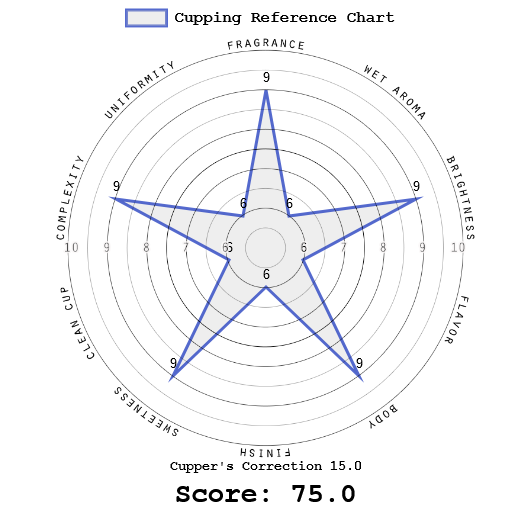
\includegraphics[width=9cm]{cupping.png} \\
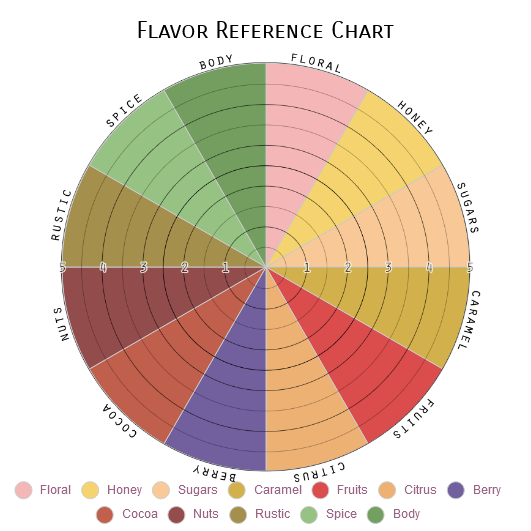
\includegraphics[width=9cm]{flavor.png}

%-------------------------------------------------------------------------------
\end{document}
